\documentclass[letterpaper, 10 pt, conference]{article} 
\usepackage[english]{babel}
\usepackage{amsmath,amssymb,amscd,amsthm} % variety of useful math macros
\usepackage[inner=1.5 cm, outer = 1.5 cm, top=1 cm, bottom = 1.5 cm]{geometry}
\usepackage{subcaption}
%For inserting graphics
\usepackage{graphicx}
\usepackage[dvipsnames]{xcolor}
\usepackage{listings}
\usepackage[utf8]{inputenc}
\usepackage{hyperref}
\usepackage{algpseudocode,algorithm}
%For diagrams
%\usepackage{tikz} 


\newcommand\N{\ensuremath{\mathcal{N}}}		%N for networks
\renewcommand{\P}{\ensuremath{\mathbb{P}}} %P for probability measures
\renewcommand{\iff}{\ensuremath{\Leftrightarrow}} %Shorter \iff 

%\newtheorem{theorem}{Theorem}
\newtheorem{prop}{Proposition}
\newtheorem{lemma}{Lemma}

\title{Generation of Poisson distributed pseudo-random numbers}
\author{G. Palafox}

\lstset{ 
	basicstyle=\footnotesize,        % the size of the fonts that are used for the code
	breakatwhitespace=false,         % sets if automatic breaks should only happen at whitespace
	breaklines=true,                 % sets automatic line breaking
	showspaces=false,                % show spaces everywhere adding particular underscores; it overrides 
	showstringspaces = false,
	stringstyle=\color{MidnightBlue},     % string literal style
	backgroundcolor=\color{White},   
}

\begin{document}

\maketitle

\begin{abstract}
Two algorithms generating Poisson-distributed pseudo-random numbers are shown. A rigorous proof for one of them is provided, while the correctness of the other one is analyzed computationally. Lastly, an example of how the binomial distribution approaches the Poisson distribution is also given.
\end{abstract}

\section{Introduction}
In this work, two algorithms for generating Poisson distributed numbers are explained. The first one assumes access to an exponentially-distributed pseudo-random number generator, while the second one assumes access to a uniformly-distributed pseudo-random number generator. Graphics and elementary probability are used to support the validity of the algorithms. In the last section, an example of how the binomial distribution approaches the Poisson distribution is given. This study was performed with R version 4.0.0 \cite{R} on a Jupyter \cite{jupyter} notebook\footnote{The notebook with the code containing our analysis, as well as this report, can be found in the Github Repository: \url{https://github.com/palafox794/AppliedProbabilityModels/tree/master/Assignment4}}. 

\section{Generating pseudo-random numbers}
First, an algorithm which generates numbers with a Poisson distribution is shown in Algorithm \ref{algo:ExpAlgo}. The idea is to generate numbers $x_i \sim \mathrm{Exp}(\lambda)$ until $x_1 + \dots + x_k$ first exceeds some number $M$. Then, we return $k - 1$. This will generate numbers following a Poisson distribution with mean $\lambda M$. A rigorous proof of this claim is not shown, however, the following intuitive explanation is given. In a Poisson process with rate $\lambda$, the number of events in an interval of length $t$ is a Poisson distributed random variable with mean $\lambda t$ \cite{Ross_2000}. Additionally, the time between events in a Poisson process is distributed exponentially with mean $1/\lambda$. From these two facts we can see that the number of exponential variables generated with sum less than $M$ must be the events occurring in a time interval of length $M$, so they must have distribution $\mathrm{Pois}(\lambda M)$. A different, significantly more informal explanation, is that if each exponential random variable is $1/\lambda$ on average,  $M \lambda$ of this variables will be needed on average for their sum to exceed $M$. 
Empirically, Figure \ref{fig:algorithm1} shows different comparisons between numbers generated by Algorithm \ref{algo:ExpAlgo} and numbers generated by R's \texttt{rpois} function with the mean we expected to see. Furthermore, R's function \texttt{MASS::fitdistr} supported our conclusions, as is seen in Table \ref{tab:fitdistr_results}.

\begin{table}[t]
	\centering
	\caption{Proposed $\lambda$ compared to $\lambda$ given by \texttt{MASS::fitdistr}}
	\begin{tabular}{l c c c}
		\hline
		 Proposed $\lambda$ & Estimated $\lambda$ by \texttt{fitdistr} & Estimated standard error\\ 
		\hline
		36 & 35.954 & 0.059 \\ 
		24 &  23.895 & 0.048 \\ 
		63 &  62.853 & 0.079 \\
		\hline
	\end{tabular}
	\label{tab:fitdistr_results}
\end{table}

 \begin{figure}
	\centering
	\begin{subfigure}[b]{0.4\linewidth}
		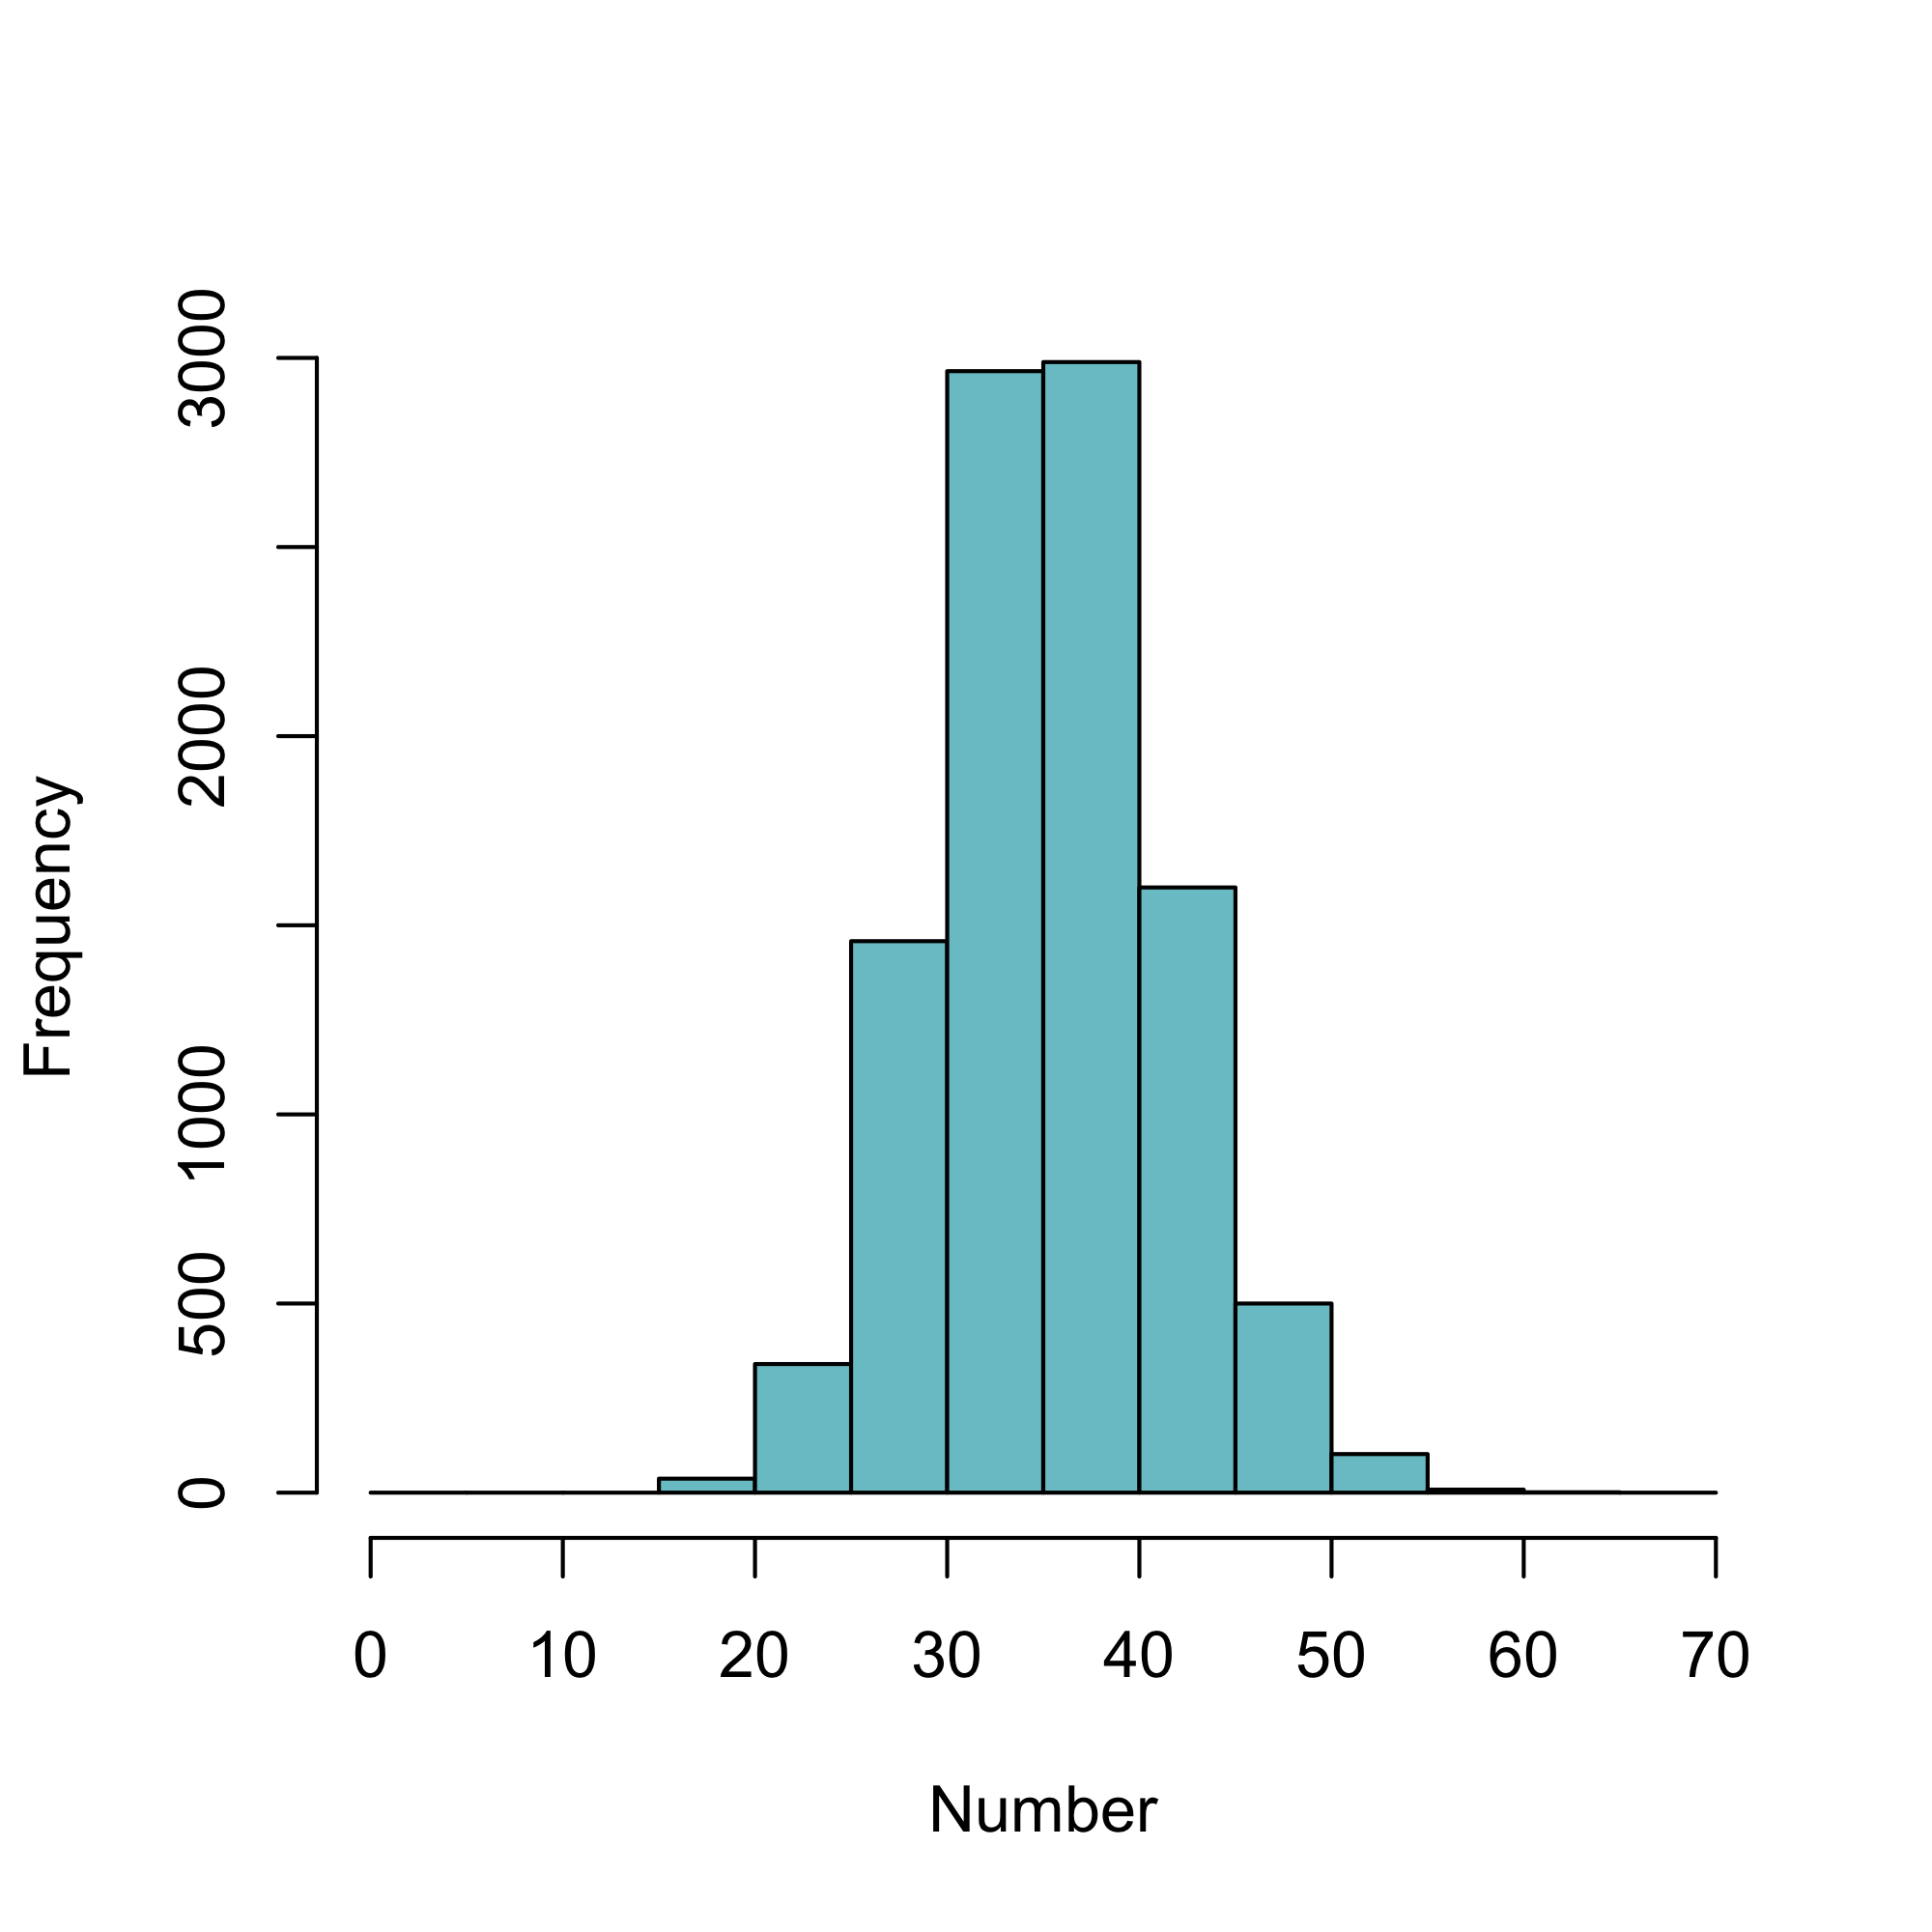
\includegraphics[width=\linewidth]{algo1_ex1.png}
		\caption{Histogram of numbers generated by Algorithm \ref{algo:ExpAlgo} with \texttt{la} = 12, \texttt{me} = 3.}
		\label{fig:algo1_ex1}
	\end{subfigure}	
	\hfill
	\begin{subfigure}[b]{0.4\linewidth}
		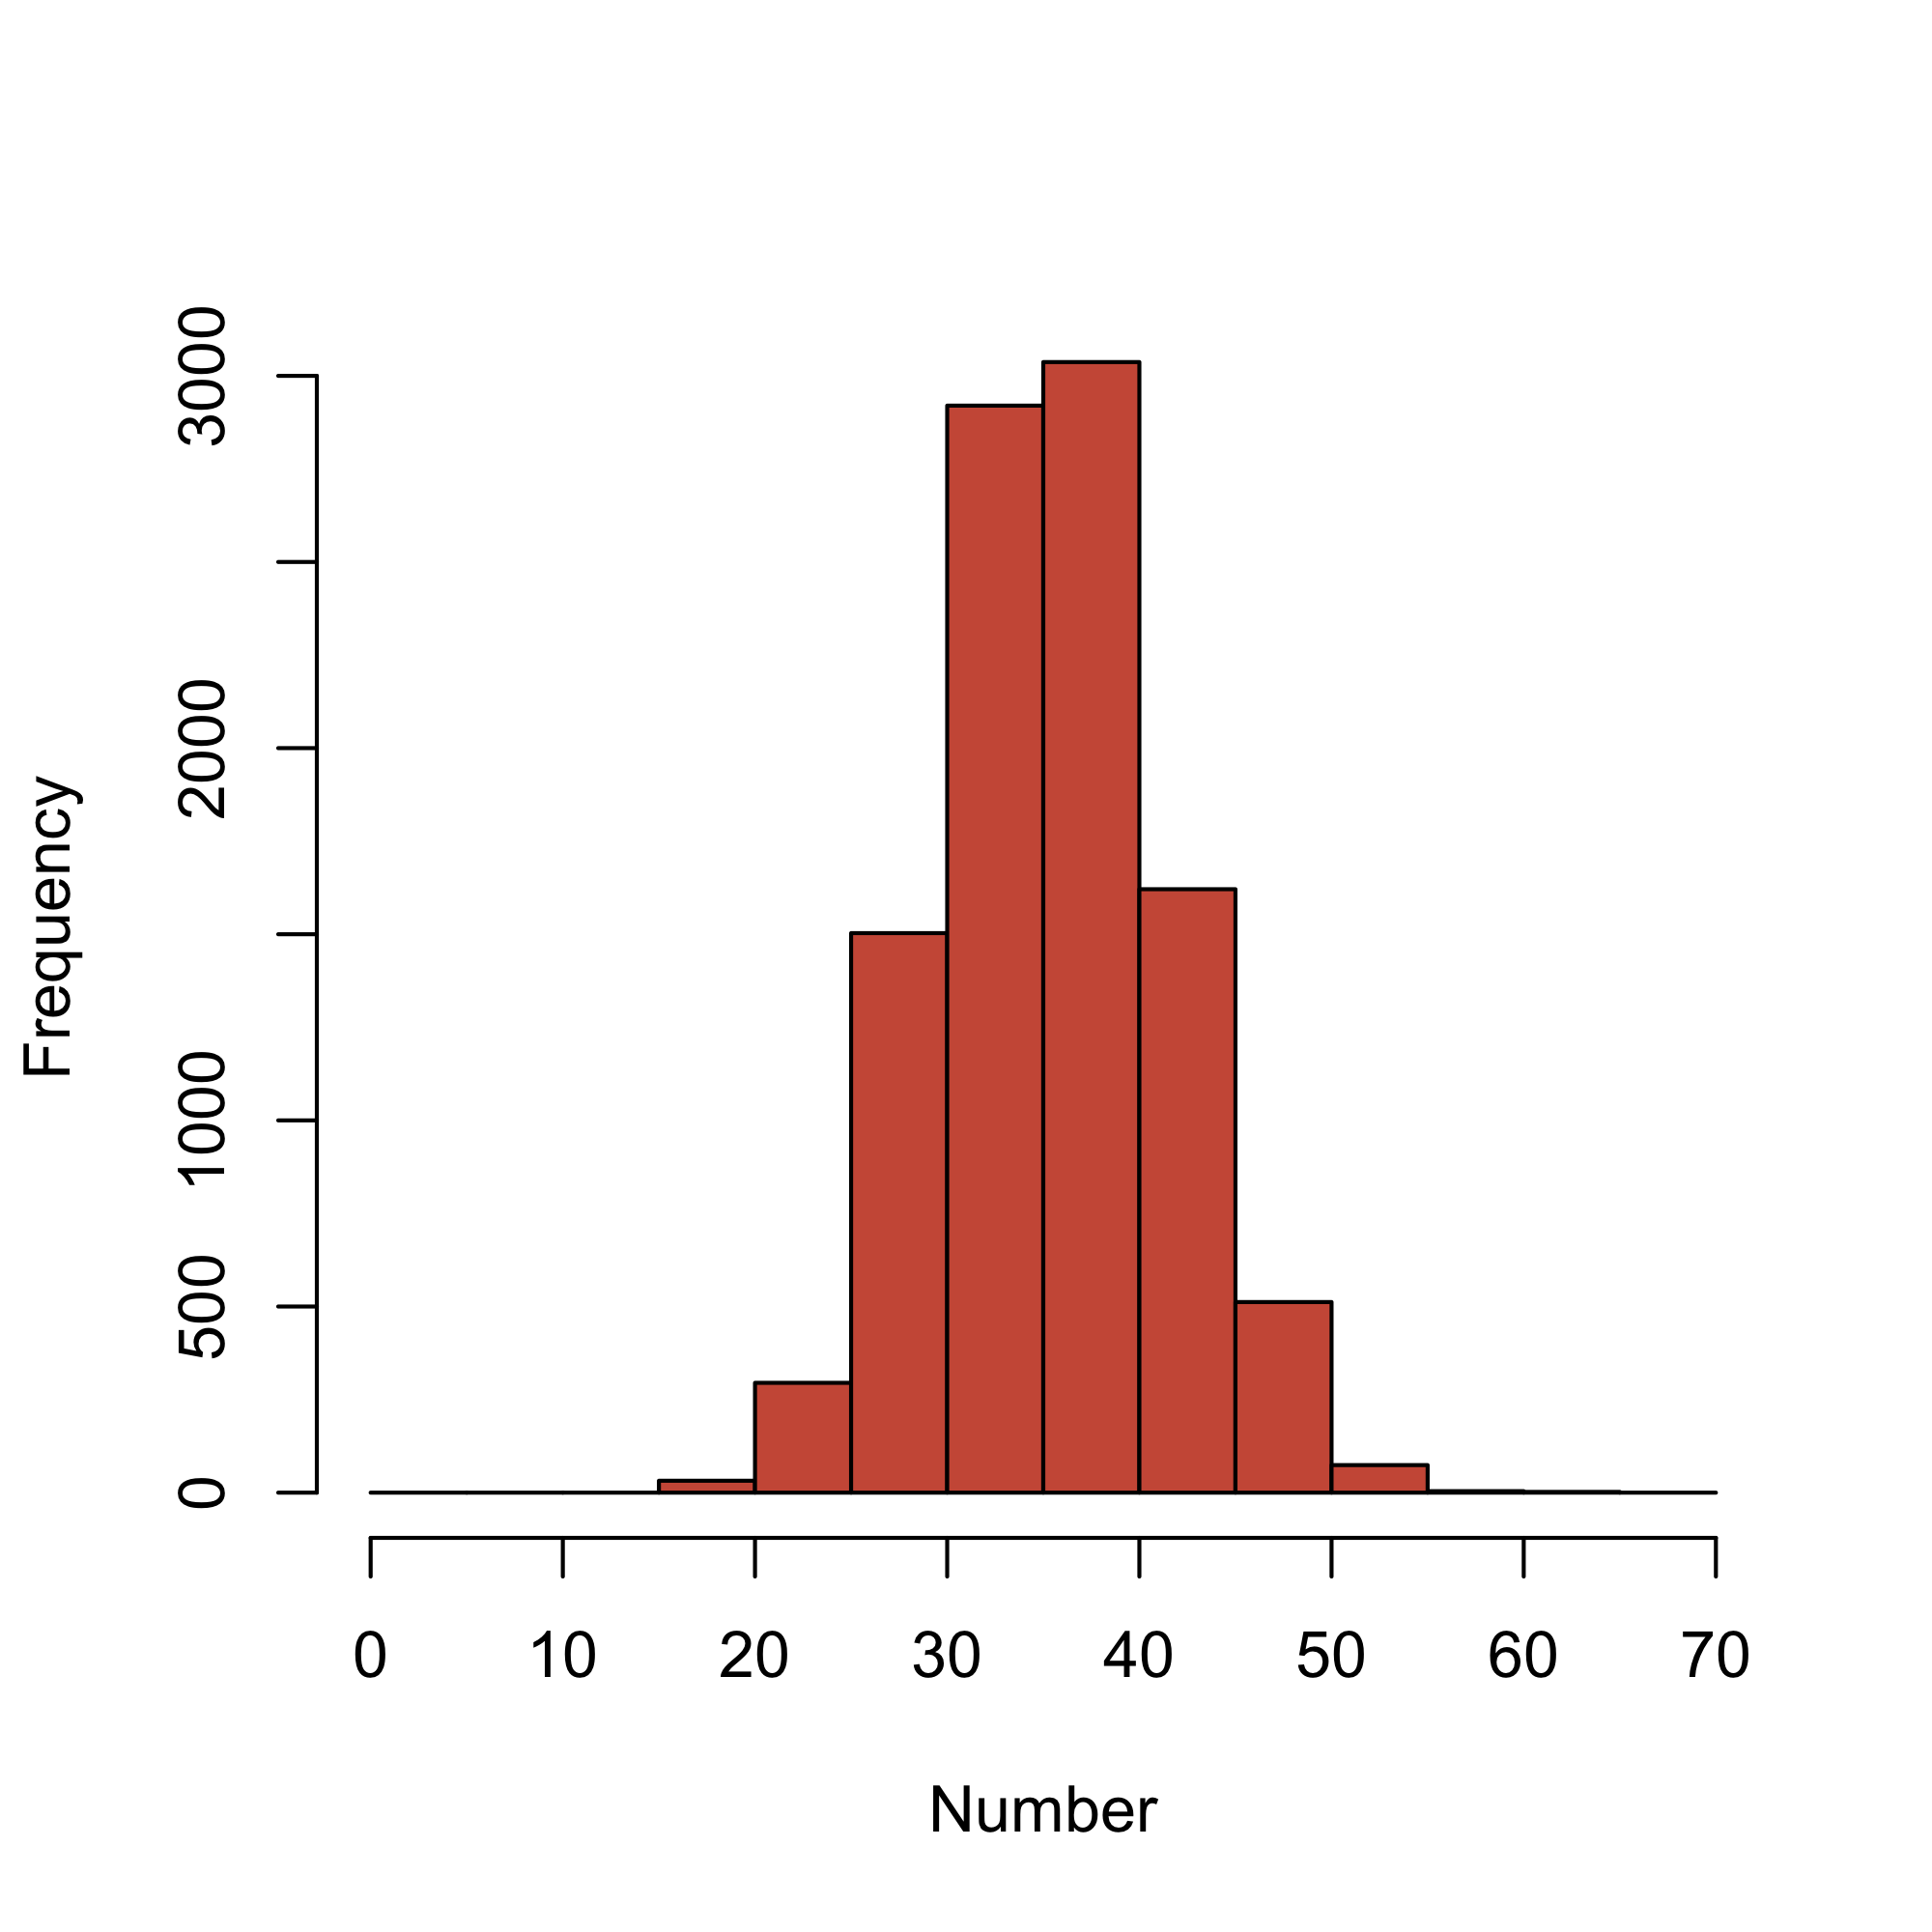
\includegraphics[width=\linewidth]{rpois_ex1.png}
		\caption{Histogram of numbers generated by R with $\mathrm{Pois}(36)$ distribution.}
		\label{fig:rpois_ex1}
	\end{subfigure}

	\begin{subfigure}[b]{0.4\linewidth}
		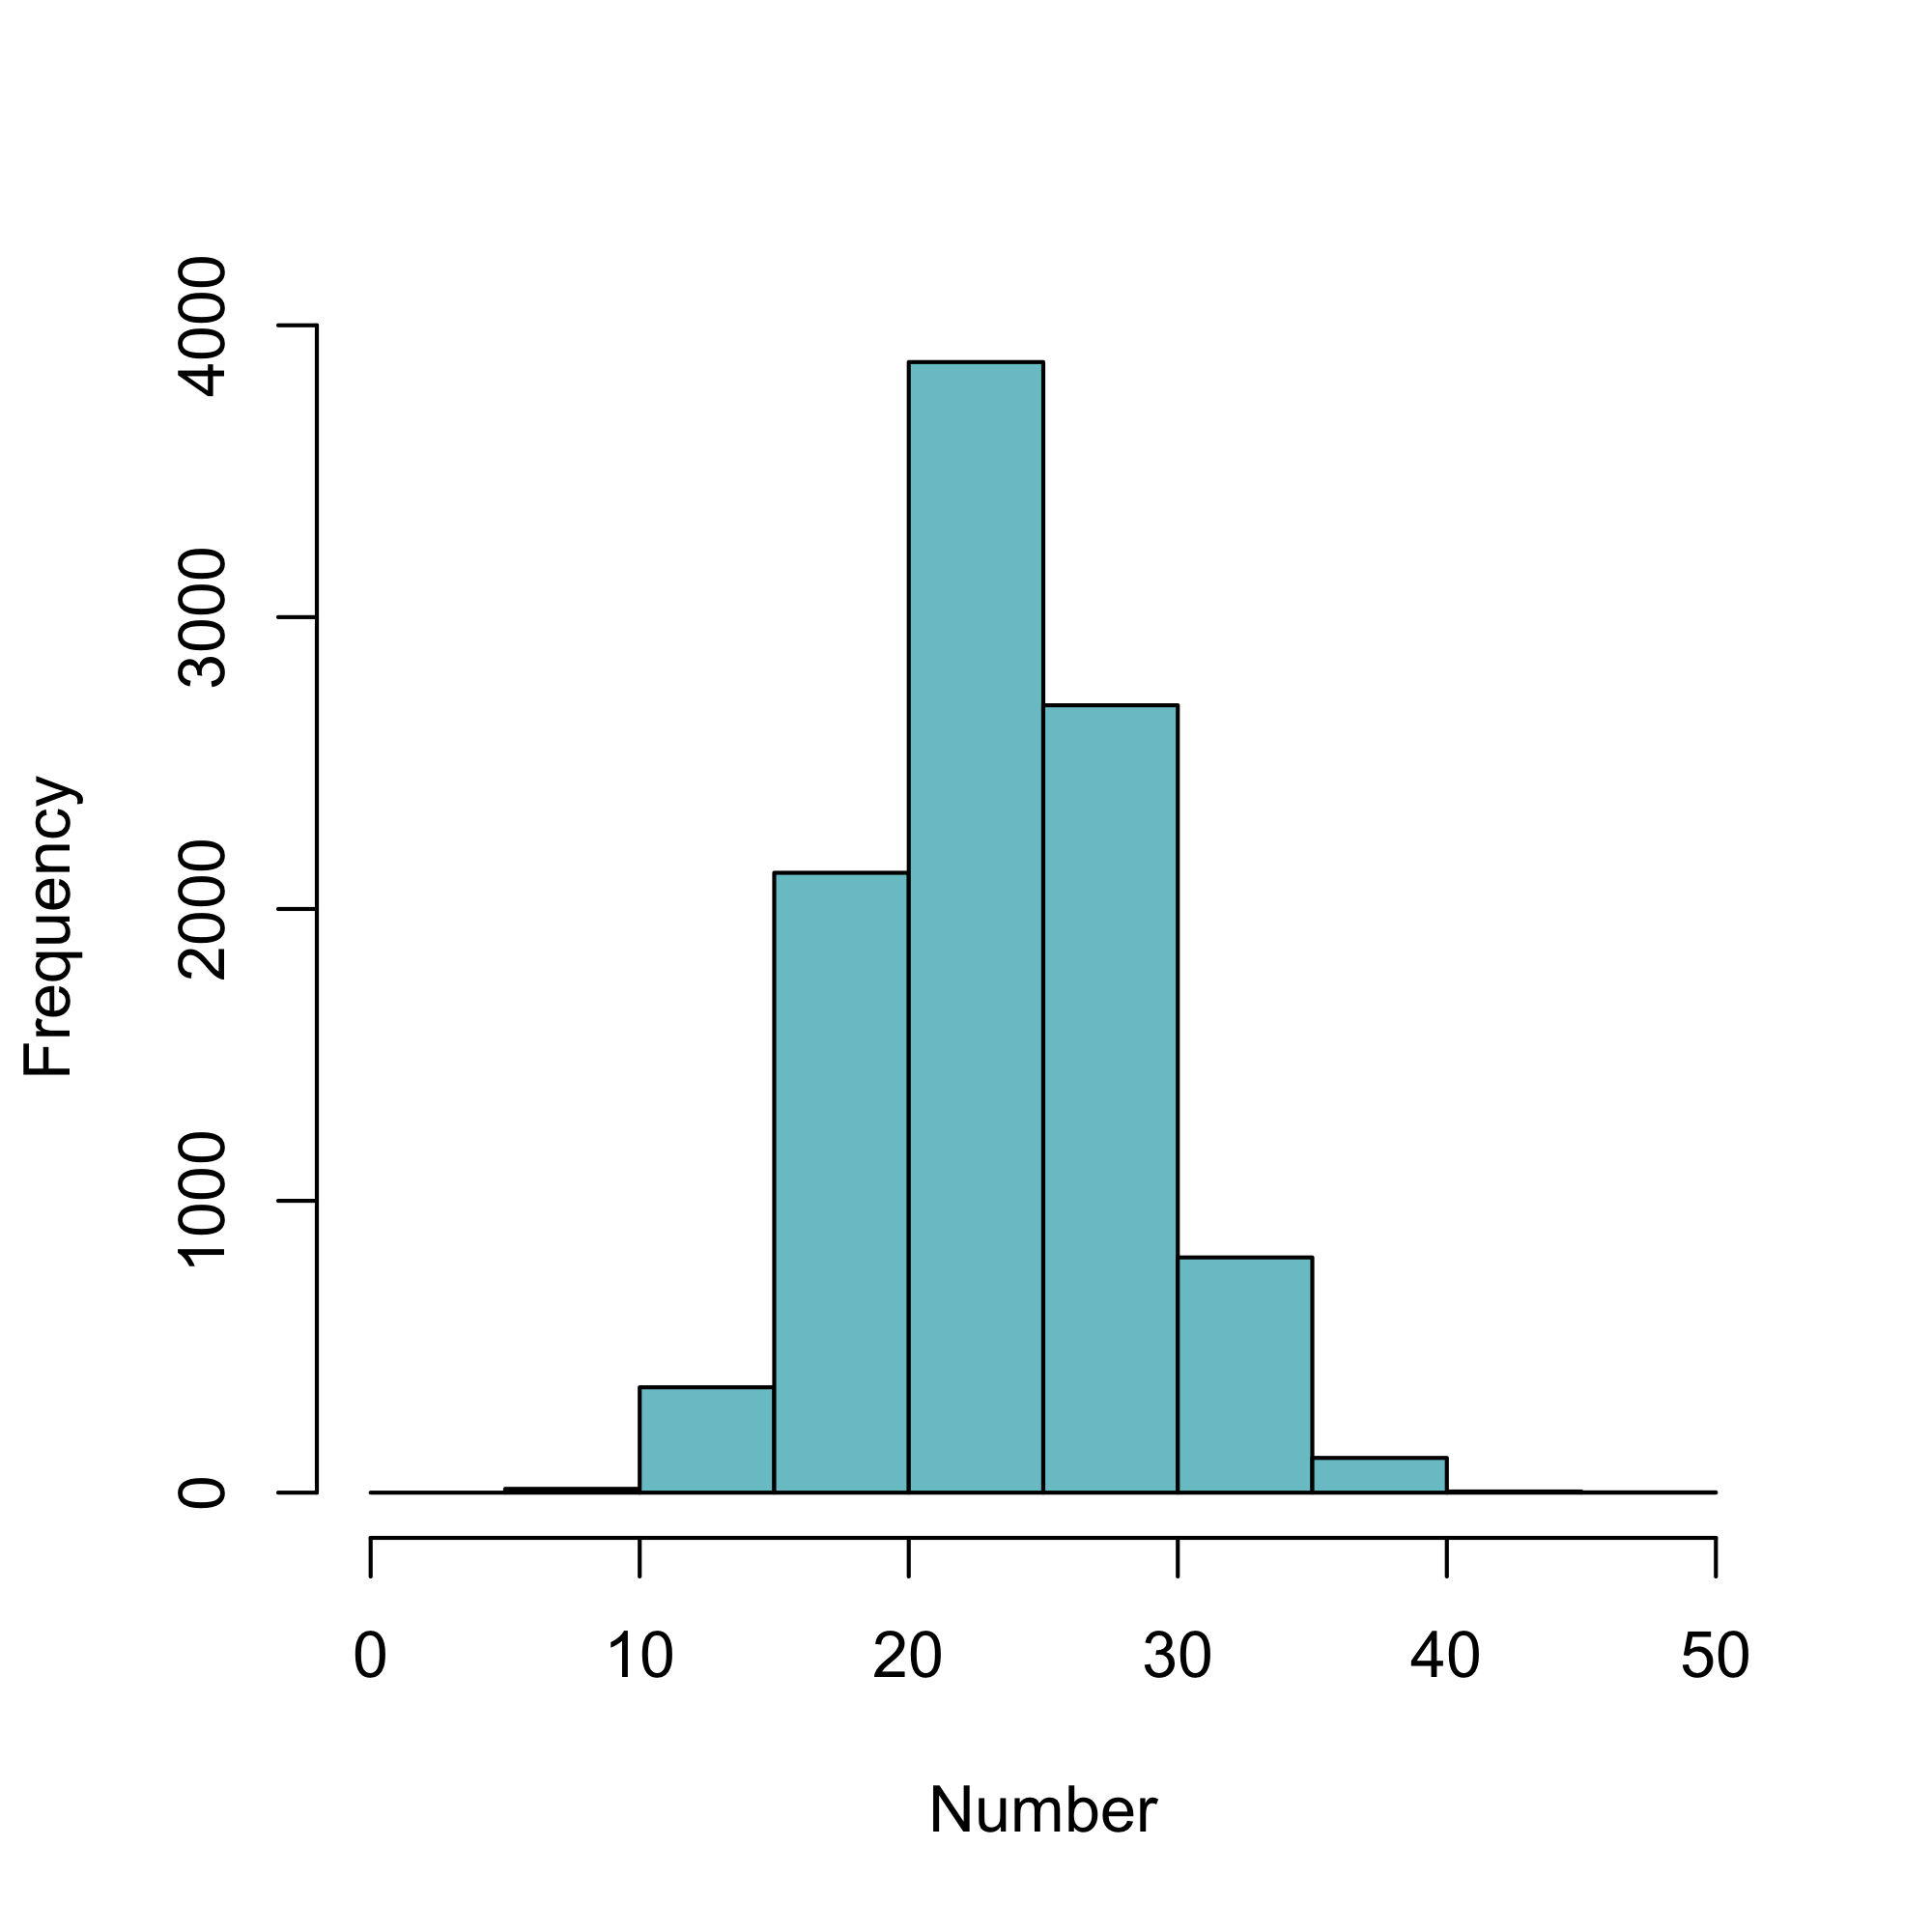
\includegraphics[width=\linewidth]{algo1_ex2.png}
		\caption{Histogram of numbers generated by Algorithm \ref{algo:ExpAlgo} with \texttt{la} = 4, \texttt{me} = 6.}
		\label{fig:algo1_ex2}
	\end{subfigure}
	\hfill
	\begin{subfigure}[b]{0.4\linewidth}
		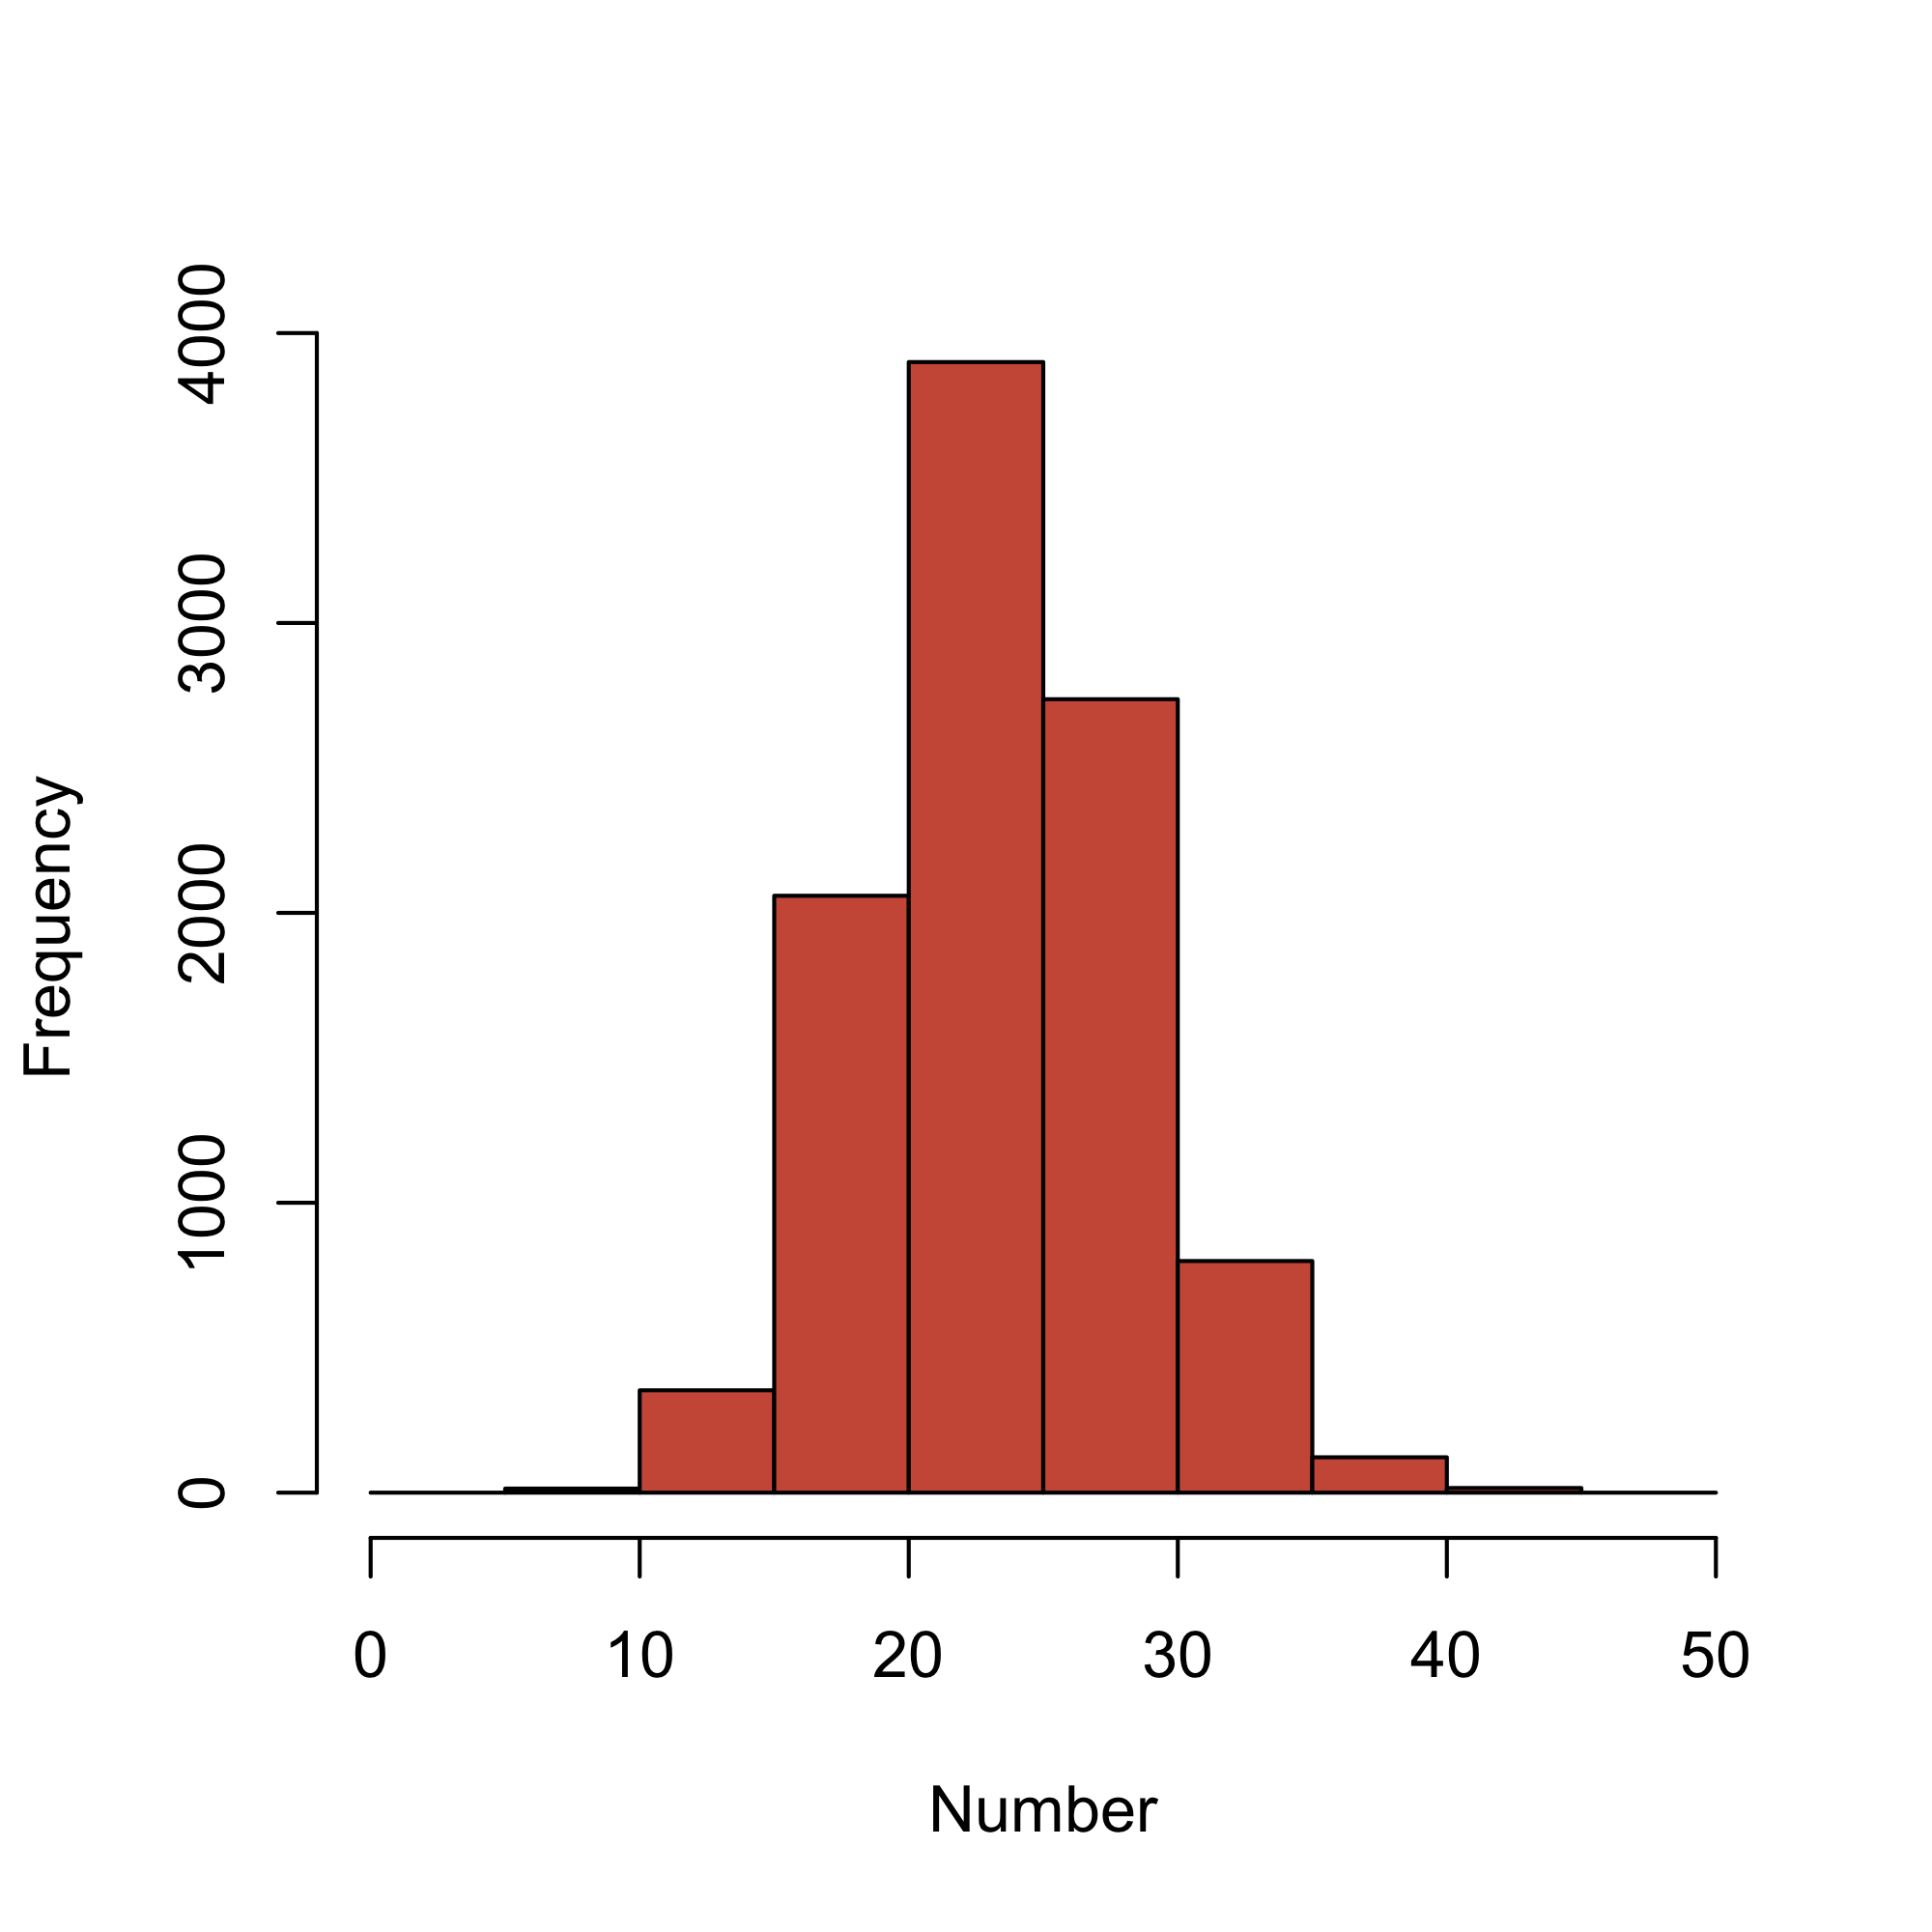
\includegraphics[width=\linewidth]{rpois_ex2.png}
		\caption{Histogram of numbers generated by R with $\mathrm{Pois}(24)$ distribution.}
		\label{fig:rpois_ex2}
	\end{subfigure}

	\begin{subfigure}[b]{0.4\linewidth}
		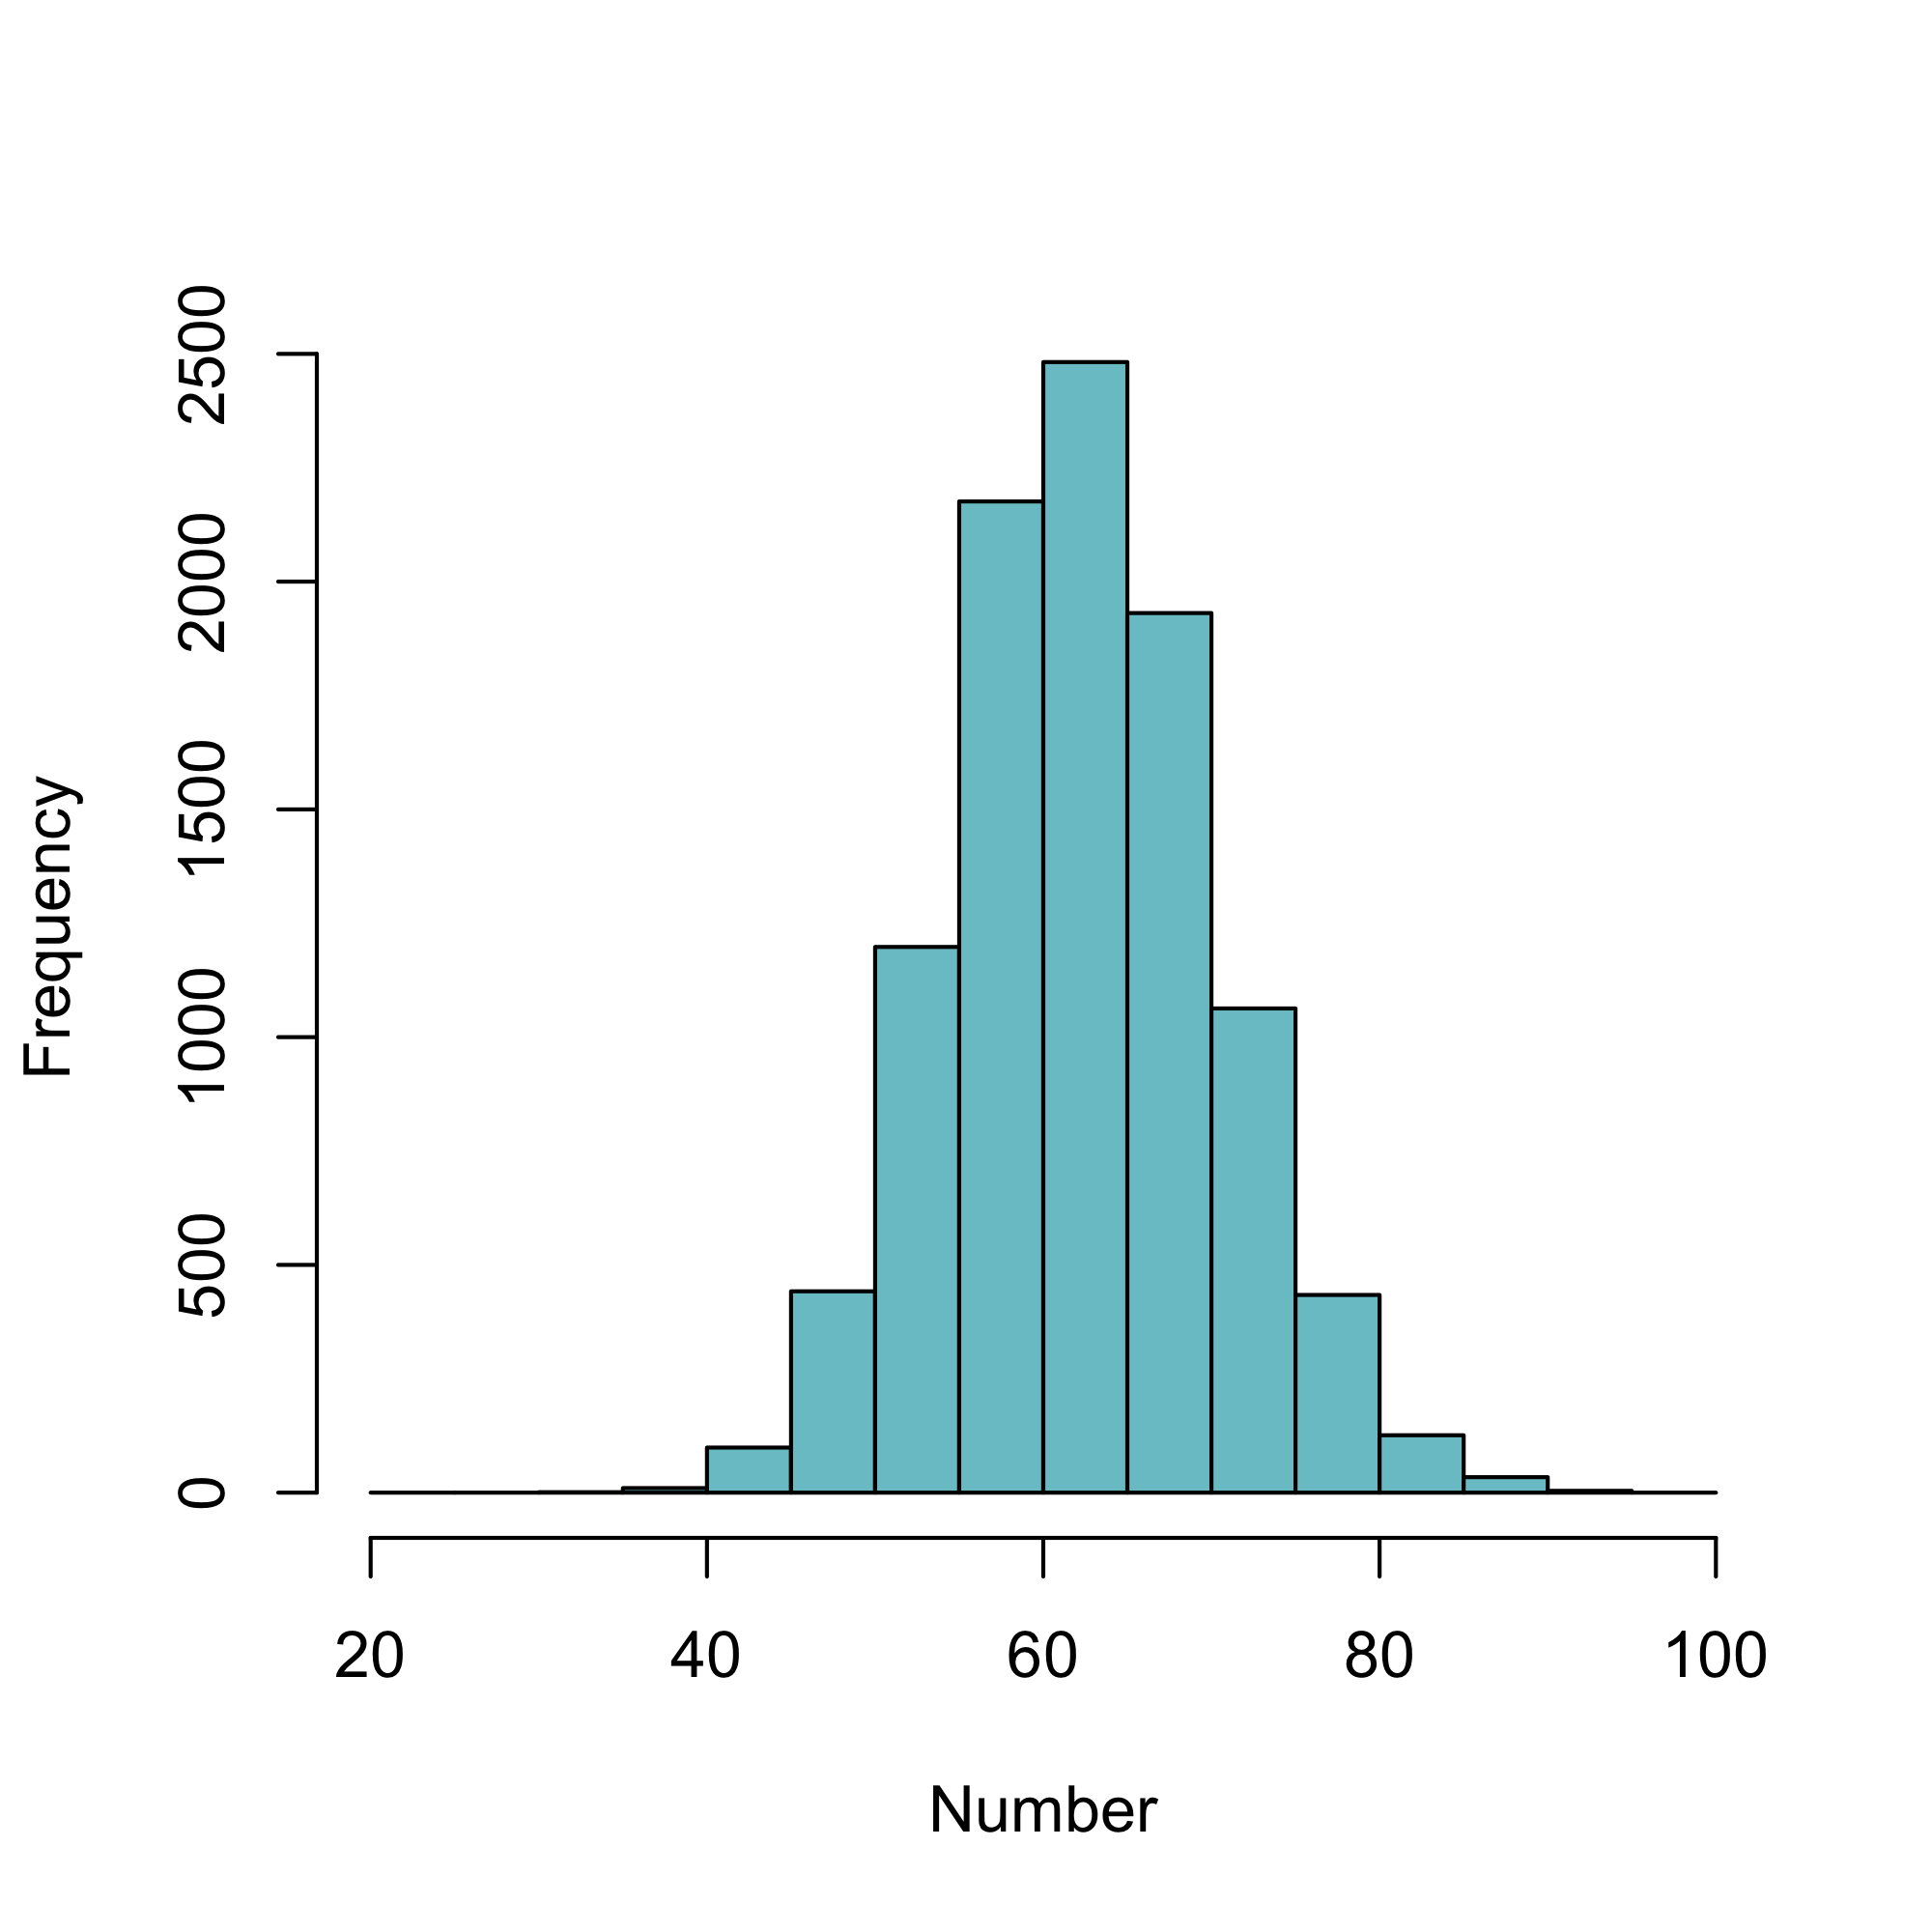
\includegraphics[width=\linewidth]{algo1_ex3.png}
		\caption{Histogram of numbers generated by Algorithm \ref{algo:ExpAlgo} with \texttt{la} = 9, \texttt{me} = 7.}
		\label{fig:algo1_ex3}
	\end{subfigure}
	\hfill
	\begin{subfigure}[b]{0.4\linewidth}
		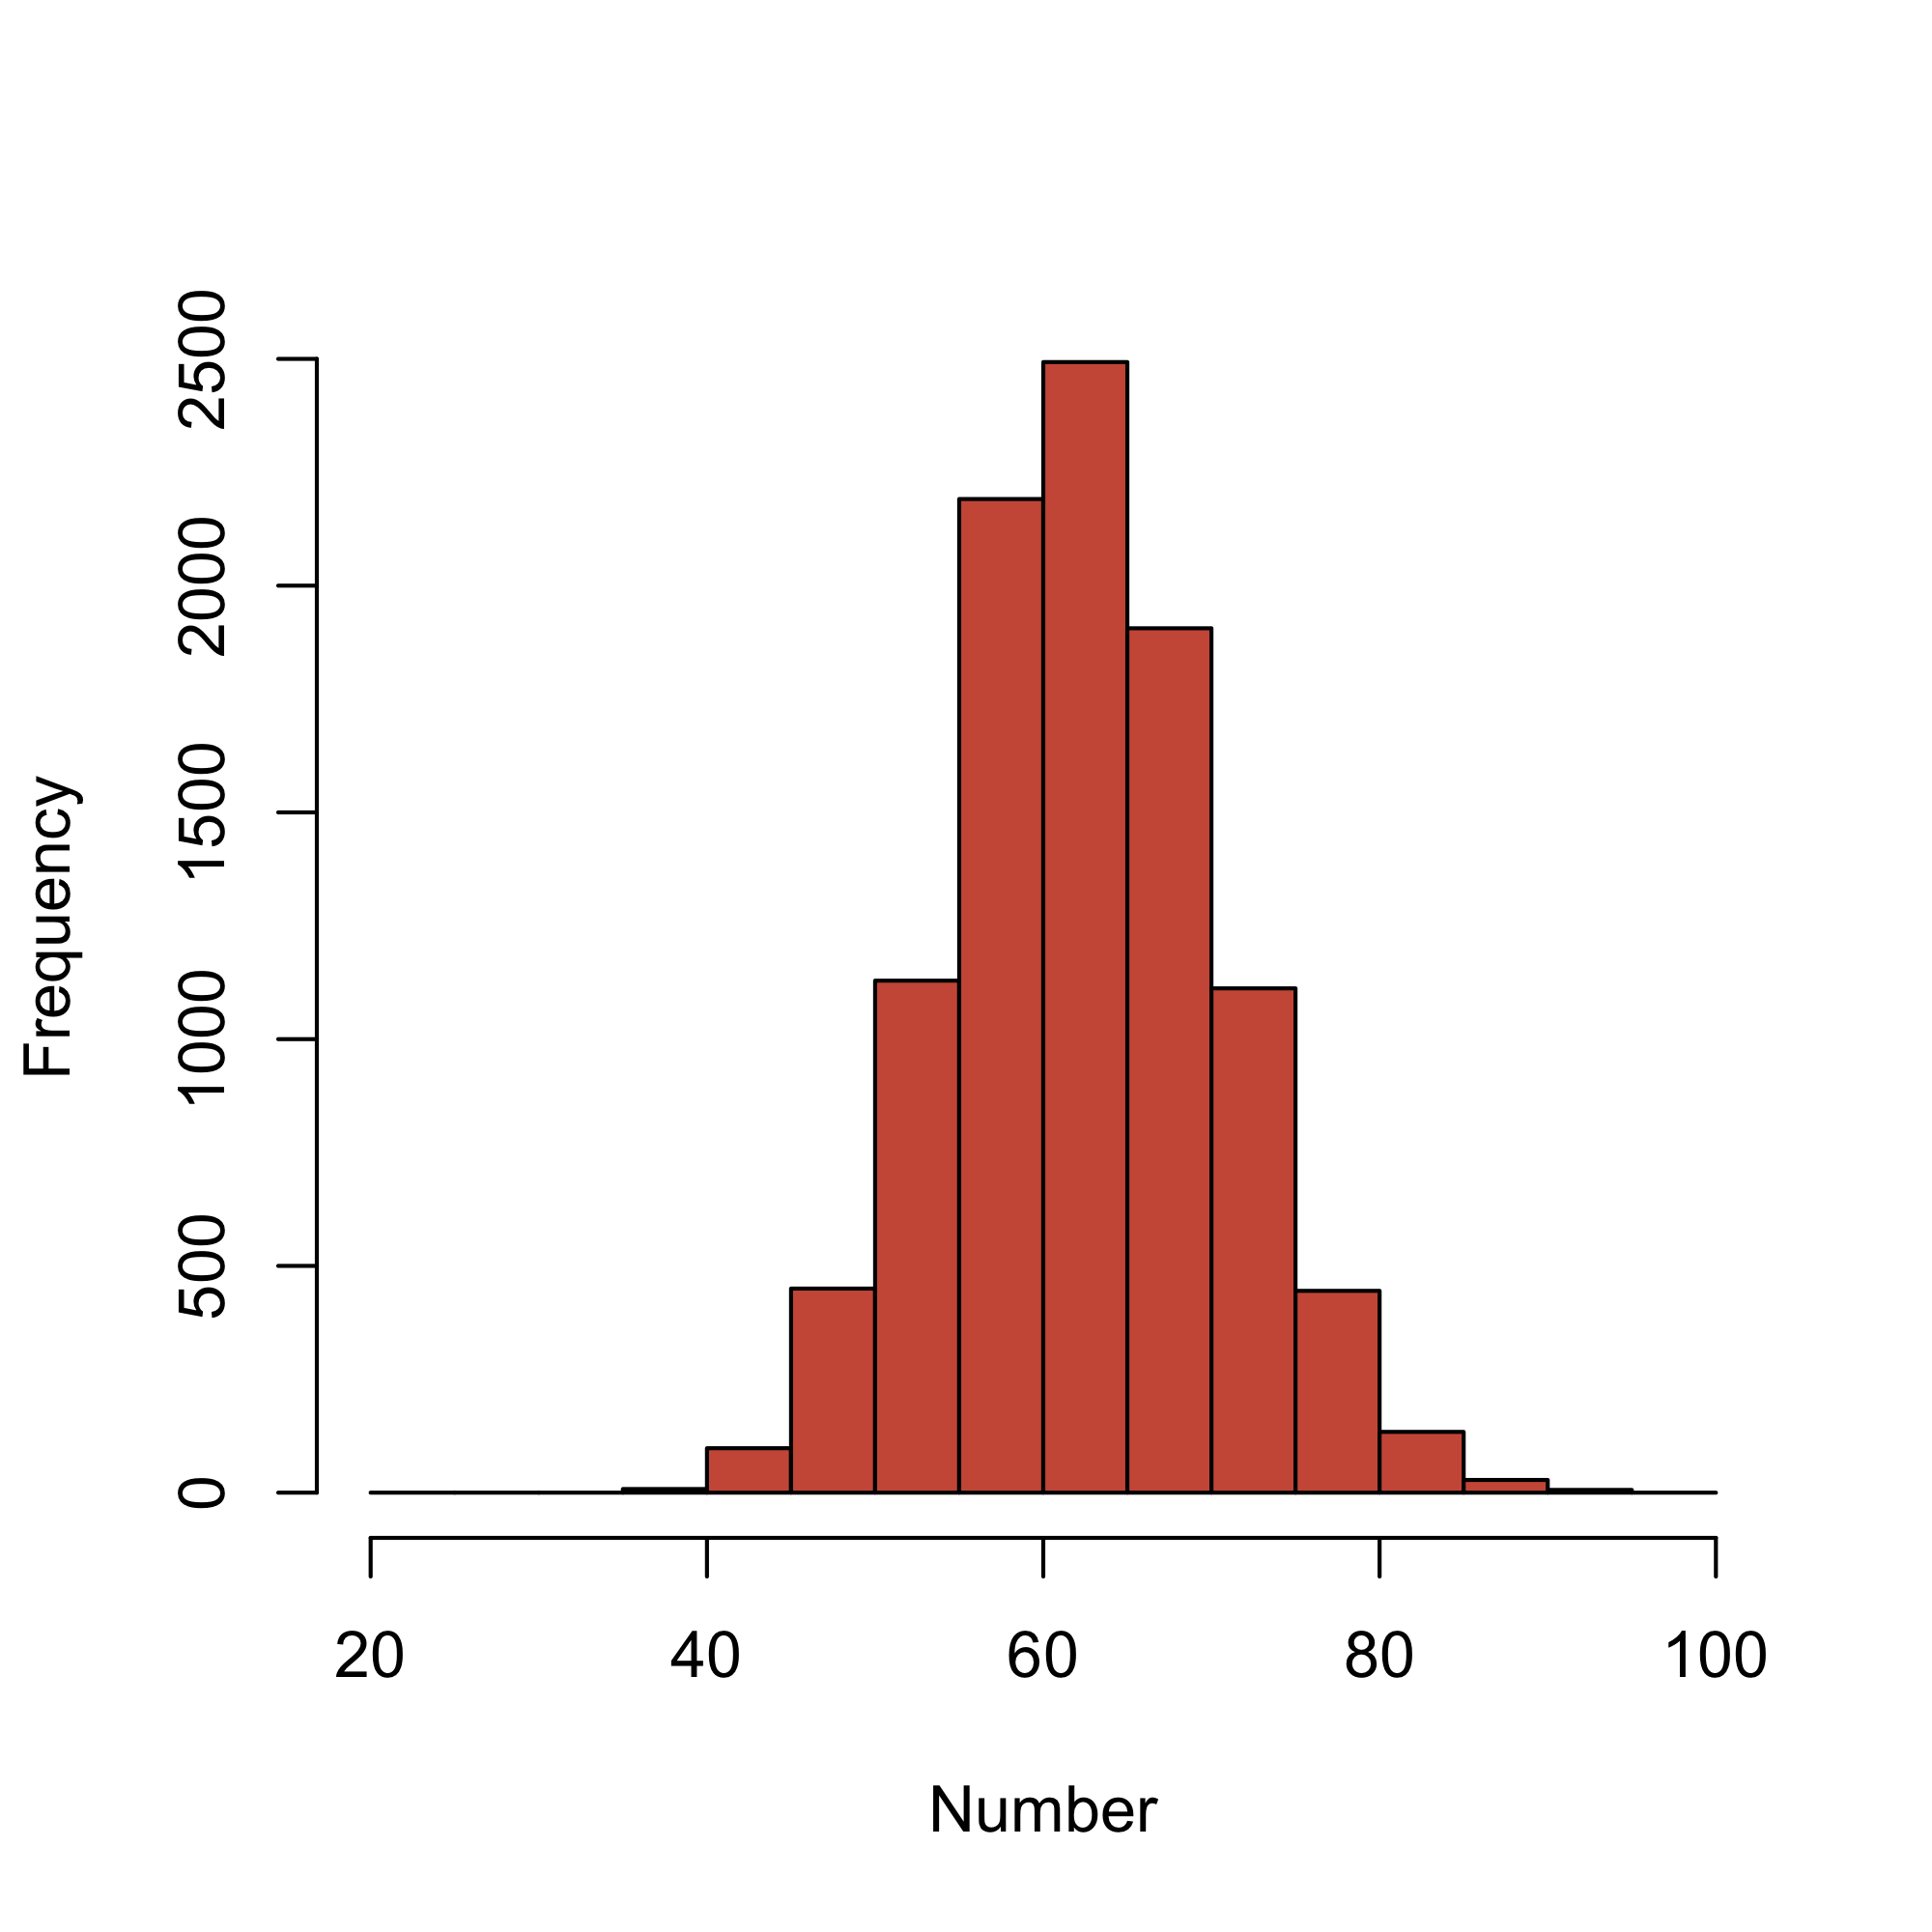
\includegraphics[width=\linewidth]{rpois_ex3.png}
	\caption{Histogram of numbers generated by R with $\mathrm{Pois}(63)$ distribution.}
		\label{fig:rpois_ex3}
	\end{subfigure}

	\caption{Comparison of Algorithm \ref{algo:ExpAlgo} vs R's generator.} 
	\label{fig:algorithm1}
\end{figure}

\begin{algorithm}
	\caption{Poisson numbers from exponentials}
	\begin{flushleft}
		\textbf{Input: } Positive values \texttt{lambda, m}; positive integer \texttt{rep}.
		\\ \textbf{Output: } Array of \texttt{rep} numbers with $\mathrm{Pois}$(\texttt{lambda} $\ast$ \texttt{m}) distribution.
	\end{flushleft}
	
	\begin{algorithmic}[1]
		\State Make empty numeric vector \texttt{ce}
		\For{\texttt{i} $=1, 2, \dots, $ \texttt{rep} }
		\State Make empty numeric vector \texttt{de}
		\While{\texttt{sum(de)} $<$ \texttt{m} }
		\State Generate pseudo-random \texttt{x} $\sim \mathrm{Exp}$(\texttt{lambda})
		\State Append \texttt{x} to array \texttt{de}
		\EndWhile
		\State Append \texttt{length(de)}-1 to array \texttt{ce}
		\EndFor
		\State \Return \texttt{ce}
	\end{algorithmic}
	\label{algo:ExpAlgo}
\end{algorithm}

\subsection{Using uniform random variables}
A different way of generating Poisson pseudo-random numbers is shown in Algorithm \ref{algo:knuth}. The algorithm is attributed to Knuth \cite{Knuth_1997}, and it can be proven as a consequence of Algorithm \ref{algo:ExpAlgo}. 

\begin{lemma}\label{lemma}
If $u \sim \mathrm{Unif}(0,1)$ and $\lambda > 0$, then $\frac{-\log(u)}{\lambda} \sim \mathrm{Exp}(\lambda)$.
\end{lemma}

\begin{proof}
First we find $\P\left(\frac{-\log(u)}{\lambda} \leq x\right)$. Observe that
\begin{align}
\frac{-\log(u)}{\lambda} \leq x &\iff -\log(u) \leq \lambda x\\
 &\iff \log(u) \geq -\lambda x\\
 &\iff u \geq \exp(-\lambda x)
\end{align}

Therefore, 
\begin{equation}
\P\left(\frac{-\log(u)}{\lambda} \leq x\right) = \P\left( u \geq \exp(-\lambda x) \right) = 1 - \P\left(u \leq \exp(-\lambda x)\right)
\end{equation}
From the cumulative distribution function for the uniform distribution, we see $\P\left(u \leq \exp(-\lambda x)\right) = \exp(-\lambda x)$, thus 
\begin{equation}
\P\left(\frac{-\log(u)}{\lambda} \leq x\right) = 1 - \exp(-\lambda x)
\end{equation}
This completes the proof.
\end{proof}

\begin{prop}
Knuth's Algorithm \ref{algo:knuth} generates pseudo-random numbers with a $\mathrm{Pois}(\lambda)$ distribution when given a parameter \texttt{lambda} = $\lambda$.
\end{prop}
\begin{proof}
We know from Algorithm \ref{algo:ExpAlgo} that counting the number of exponential random variables with mean $1/\lambda$ such that $x_1 + \dots + x_k < 1$ gives us a Poisson variable with mean $\lambda$.
Using Lemma \ref{lemma} we can rewrite this as $-\frac{\log(u_1)}{\lambda} - \dots - \frac{\log(u_k)}{\lambda} < 1$, where $u_i \sim \mathrm{Unif}(0,1)$. Then, observe that
\begin{align}
-\frac{\log(u_1)}{\lambda} - \dots - \frac{\log(u_k)}{\lambda} < 1 &\iff -\log(u_1) - \dots - \log(u_k) < \lambda \\
&\iff -\log(u_1 u_2 \cdots u_k) < \lambda \\
&\iff u_1 u_2 \cdots u_k > \exp(-\lambda)
\end{align}
This shows that the number of exponential random variables generated before its sum exceeds one is the same as the number of uniform random variables generated before its product is less than $\exp(-\lambda)$ and so they must have the same distribution.
\end{proof}

Supporting the formal proof, a comparison of numbers generated by Algorithm \ref{algo:knuth} and by R's \texttt{rpois} function is shown in Figure \ref{fig:algorithm2}.

 \begin{figure}
	\centering
	\begin{subfigure}[b]{0.45\linewidth}
		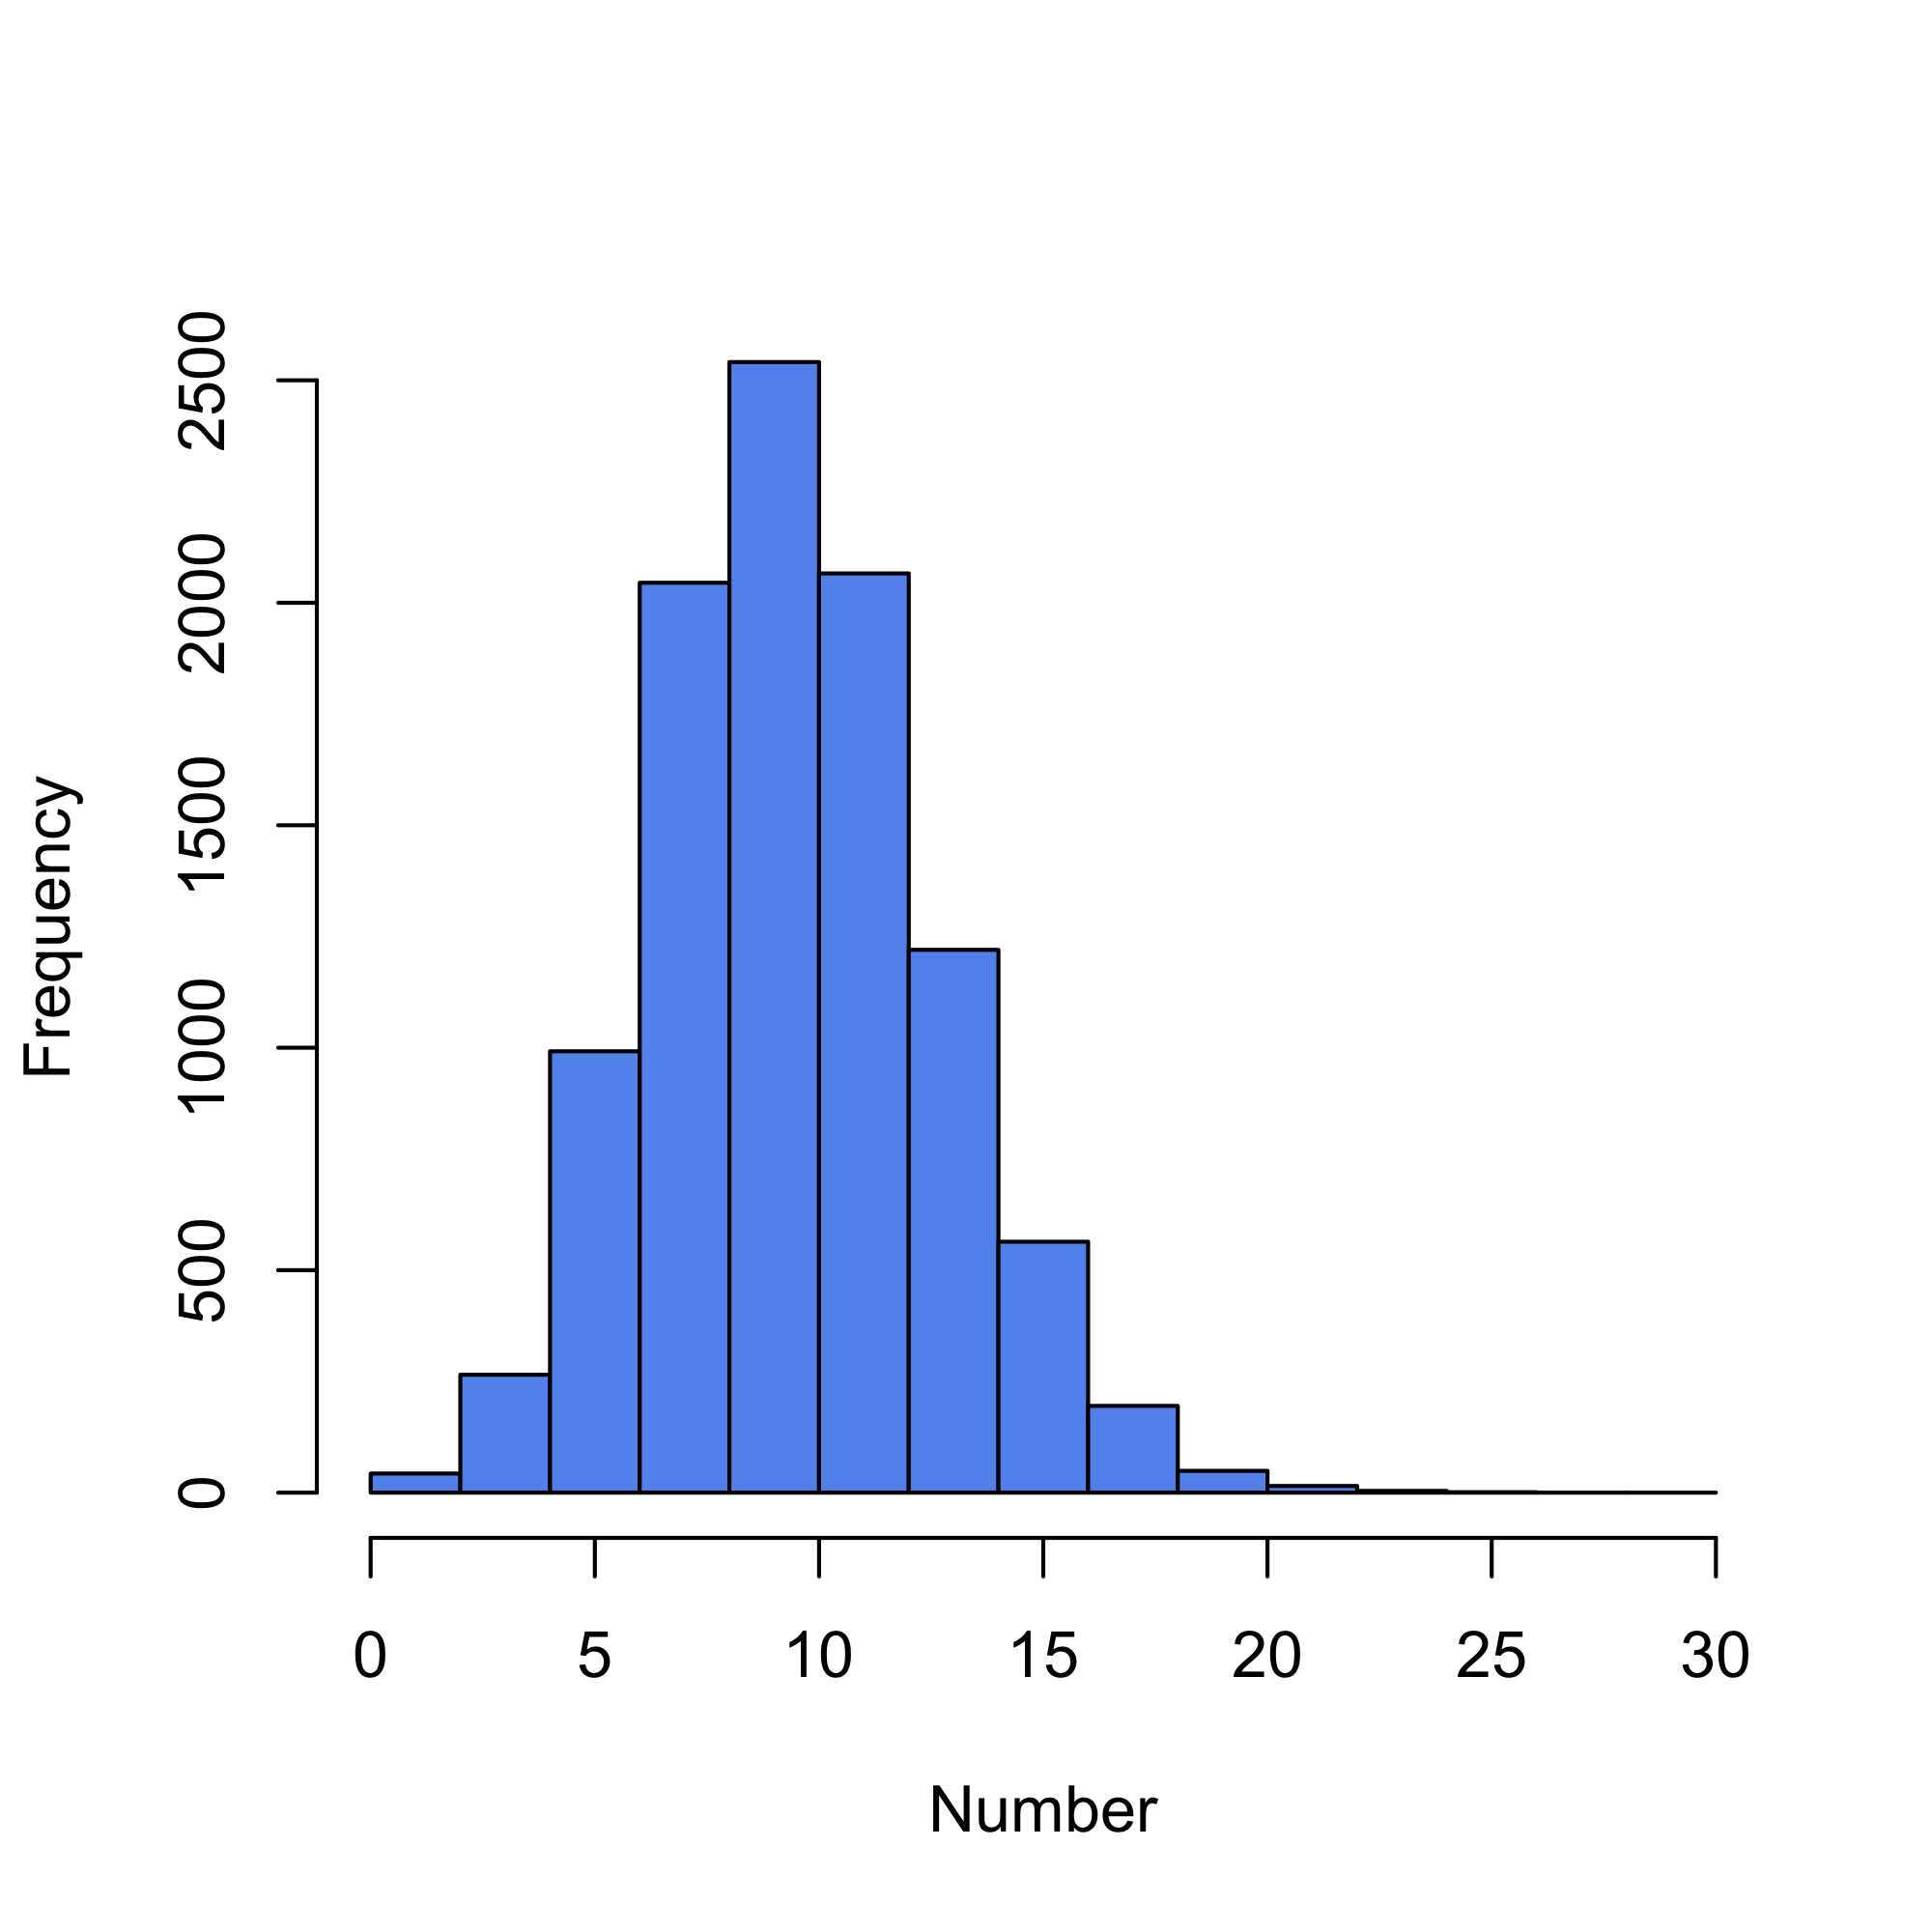
\includegraphics[width=\linewidth]{knuth_algo.png}
		\caption{Histogram of numbers generated by Algorithm \ref{algo:knuth} with \texttt{la} = 10.}
		\label{fig:knuth_algo}
	\end{subfigure}
	\hfill
	\begin{subfigure}[b]{0.45\linewidth}
		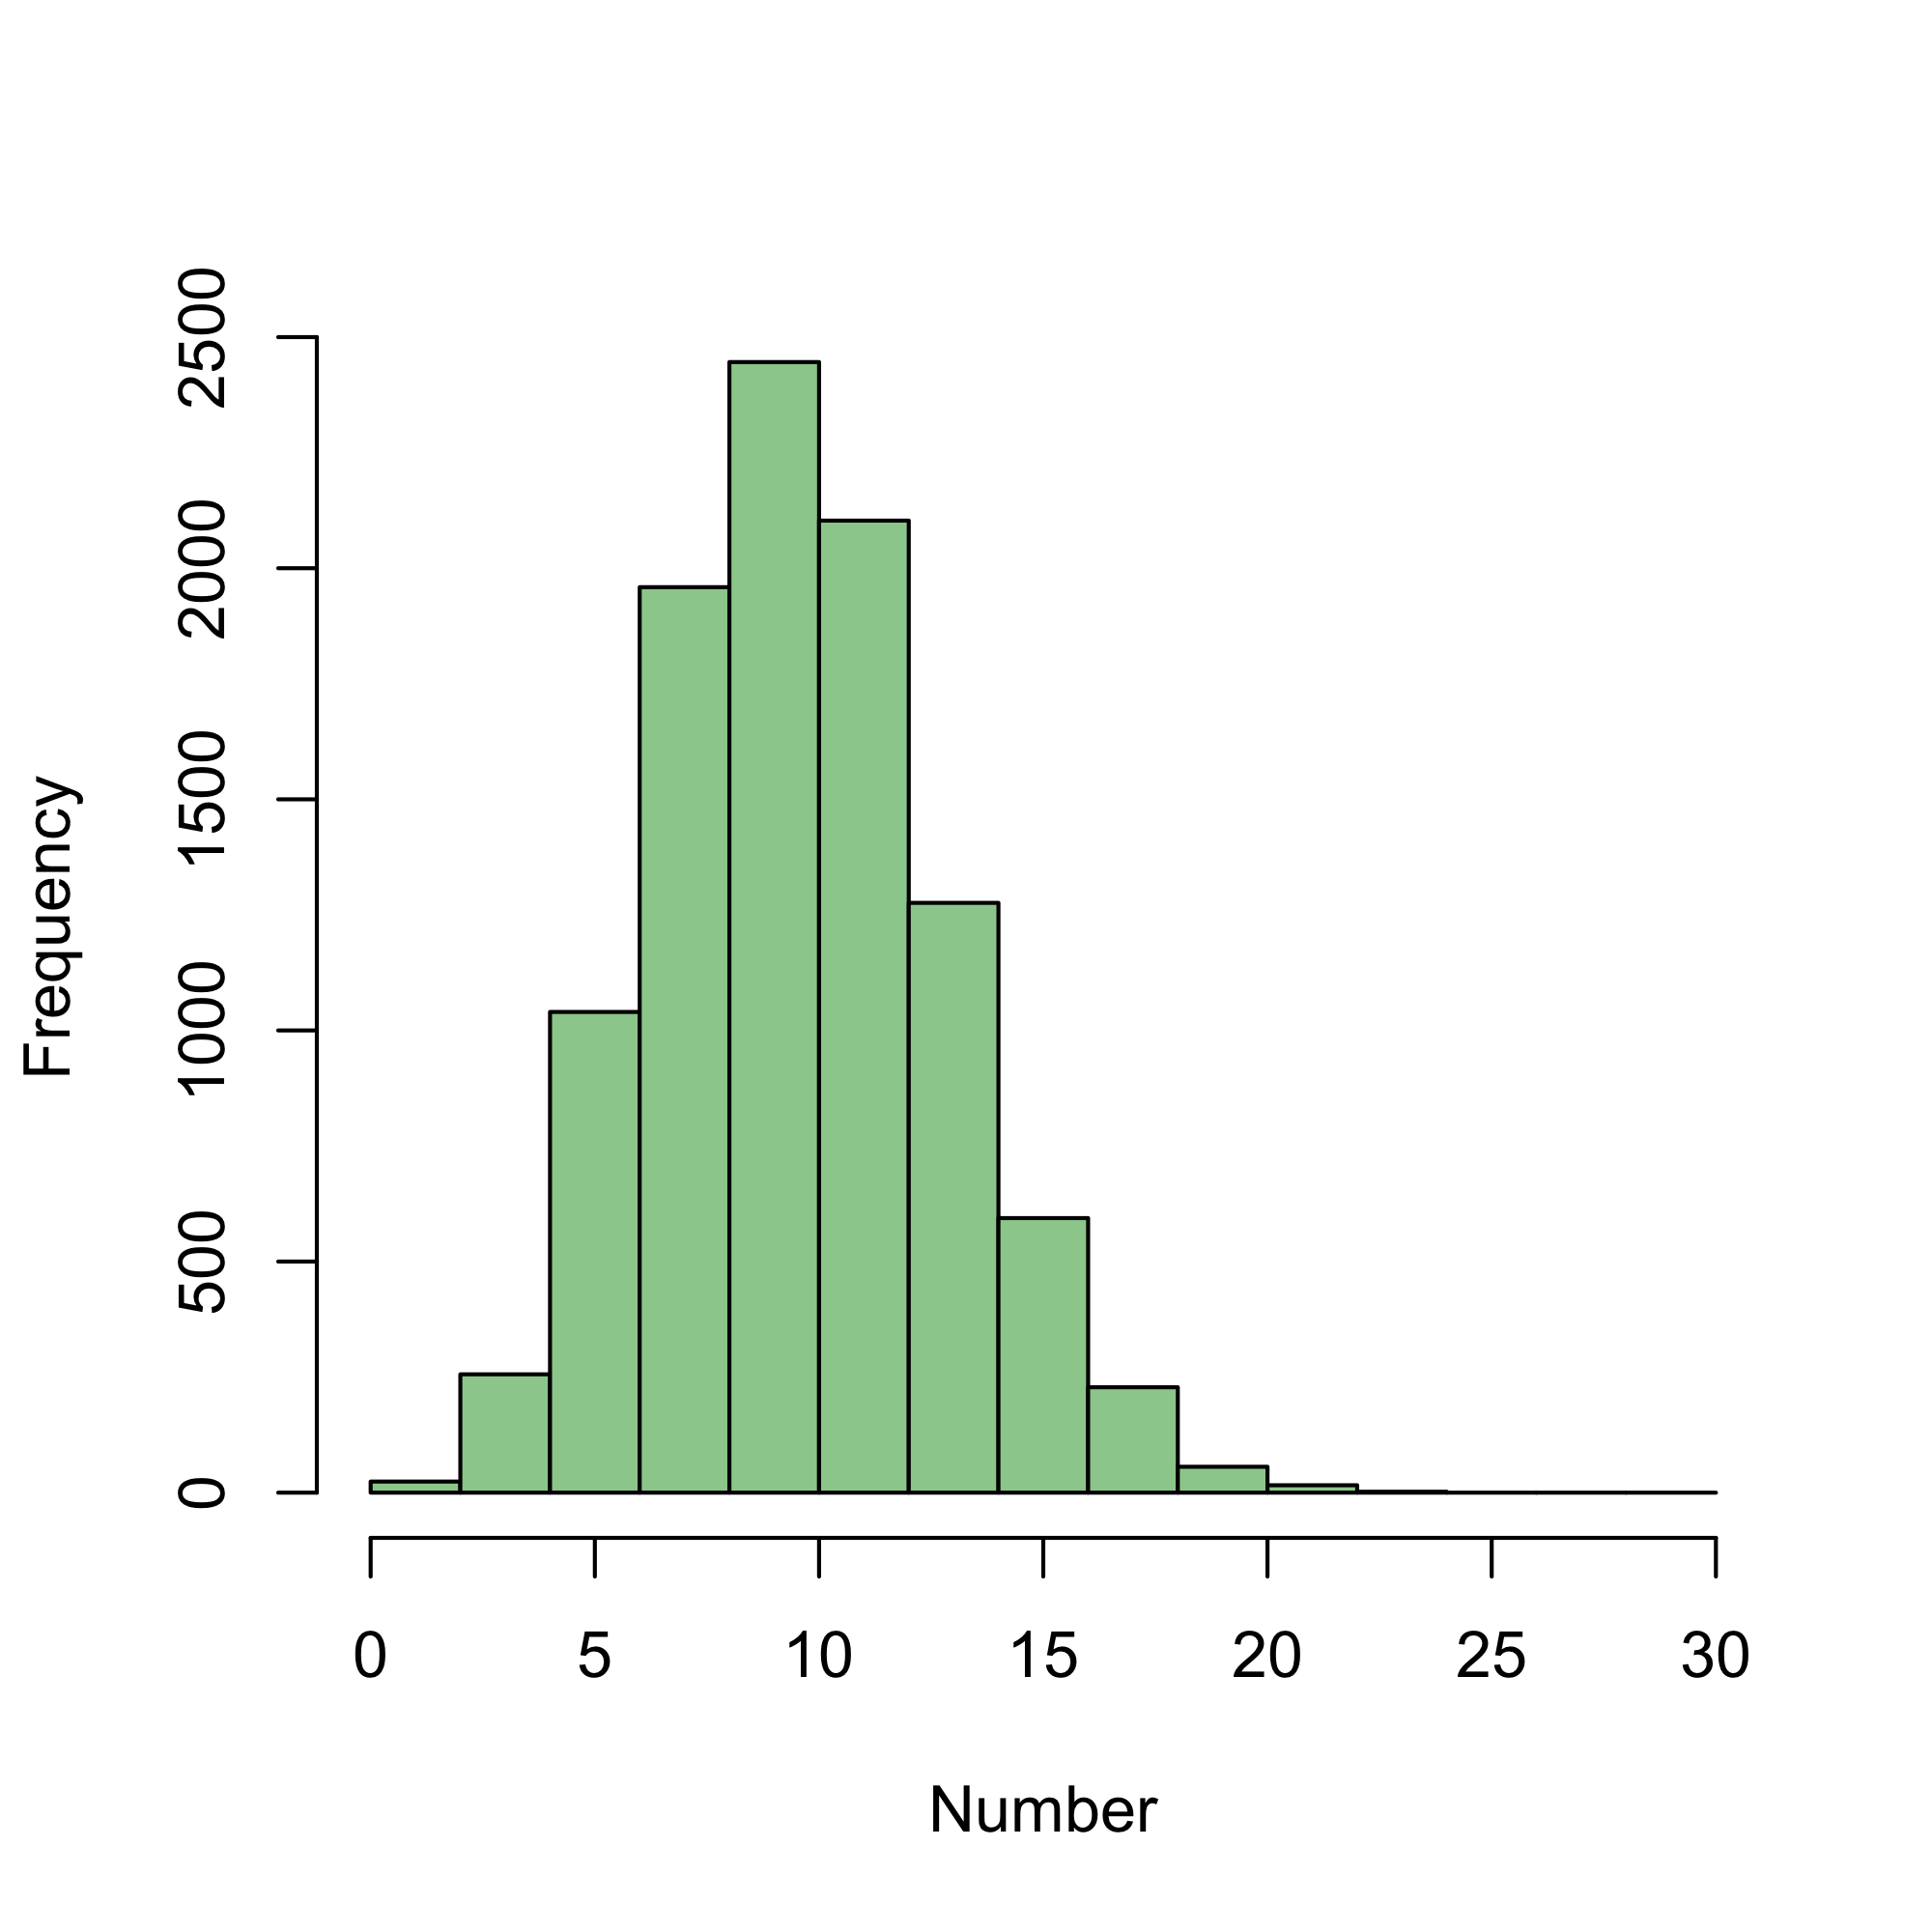
\includegraphics[width=\linewidth]{rpois_knuth.png}
		\caption{Histogram of numbers generated by R with $\mathrm{Pois}(10)$ distribution.}
		\label{fig:rpois_knuth}
	\end{subfigure}
	\caption{Comparison of Algorithm \ref{algo:knuth} vs R's generator.} 
	\label{fig:algorithm2}
\end{figure}


\begin{algorithm}
	\caption{Knuth's algorithm}
	\begin{flushleft}
		\textbf{Input: } Positive value \texttt{lambda}; positive integer \texttt{rep}.
		\\ \textbf{Output: } Array of \texttt{rep} numbers with $\mathrm{Pois}$(\texttt{lambda}) distribution.
	\end{flushleft}
	
	\begin{algorithmic}[1]
		\State Make empty numeric vector \texttt{cu}
		\For{\texttt{i} $=1, 2, \dots, $ \texttt{rep} }
		\State Make a numeric vector \texttt{du} containing only value 1
		\While{\texttt{prod(du)} $>$ \texttt{exp(-lambda)} }
		\State Generate pseudo-random \texttt{u} $\sim$ \texttt{Unif(0,1)}
		\State Append \texttt{u} to array \texttt{du}
		\EndWhile
		\State Append \texttt{length(du)}-2 to array \texttt{cu}
		\EndFor
		\State \Return \texttt{cu}
	\end{algorithmic}
	\label{algo:knuth}
\end{algorithm}

\section{Binomial distribution tends to Poisson distribution}
It is known \cite{Ross_1976} that for $n$ large and small $p$, the binomial distribution $\mathrm{Binom}(n, p)$ can be approximated with a Poisson distribution $\mathrm{Pois}(np)$. This situation is exemplified with a random graph. An Erdős–Rényi random network \cite{newman}, denoted as $G(n, p)$, is defined in the following way: $n$ nodes are fixed, and an edge is placed between each distinct pair with independent probability $p$. It should be clear that the probability of any vertex having degree $k$ is ${n-1 \choose k} p^k (1-p)^{n-1-k}$. That is, the degree of vertices has a binomial distribution. A random network $G(10 000, \frac{1}{10 000})$ is created using R's library \texttt{igraph}. The degree distribution of this network is binomial, due to the justification given above. However, since $n$ is sufficiently large and $p$ is sufficiently small, the degree distribution can be approximated as a Poisson distribution. Figure \ref{fig:gnp_degree_histogram} shows the degree distribution of the network, and Figure \ref{fig:poiss_aprox_binomial} shows an identical histogram for numbers having a $\mathrm{Pois}(1)$ distribution. Figure \ref{fig:gnp_vs_poiss_boxplot} shows a boxplot comparing these two sets of data.

\begin{figure}
	\centering
	\begin{subfigure}[b]{0.45\linewidth}
		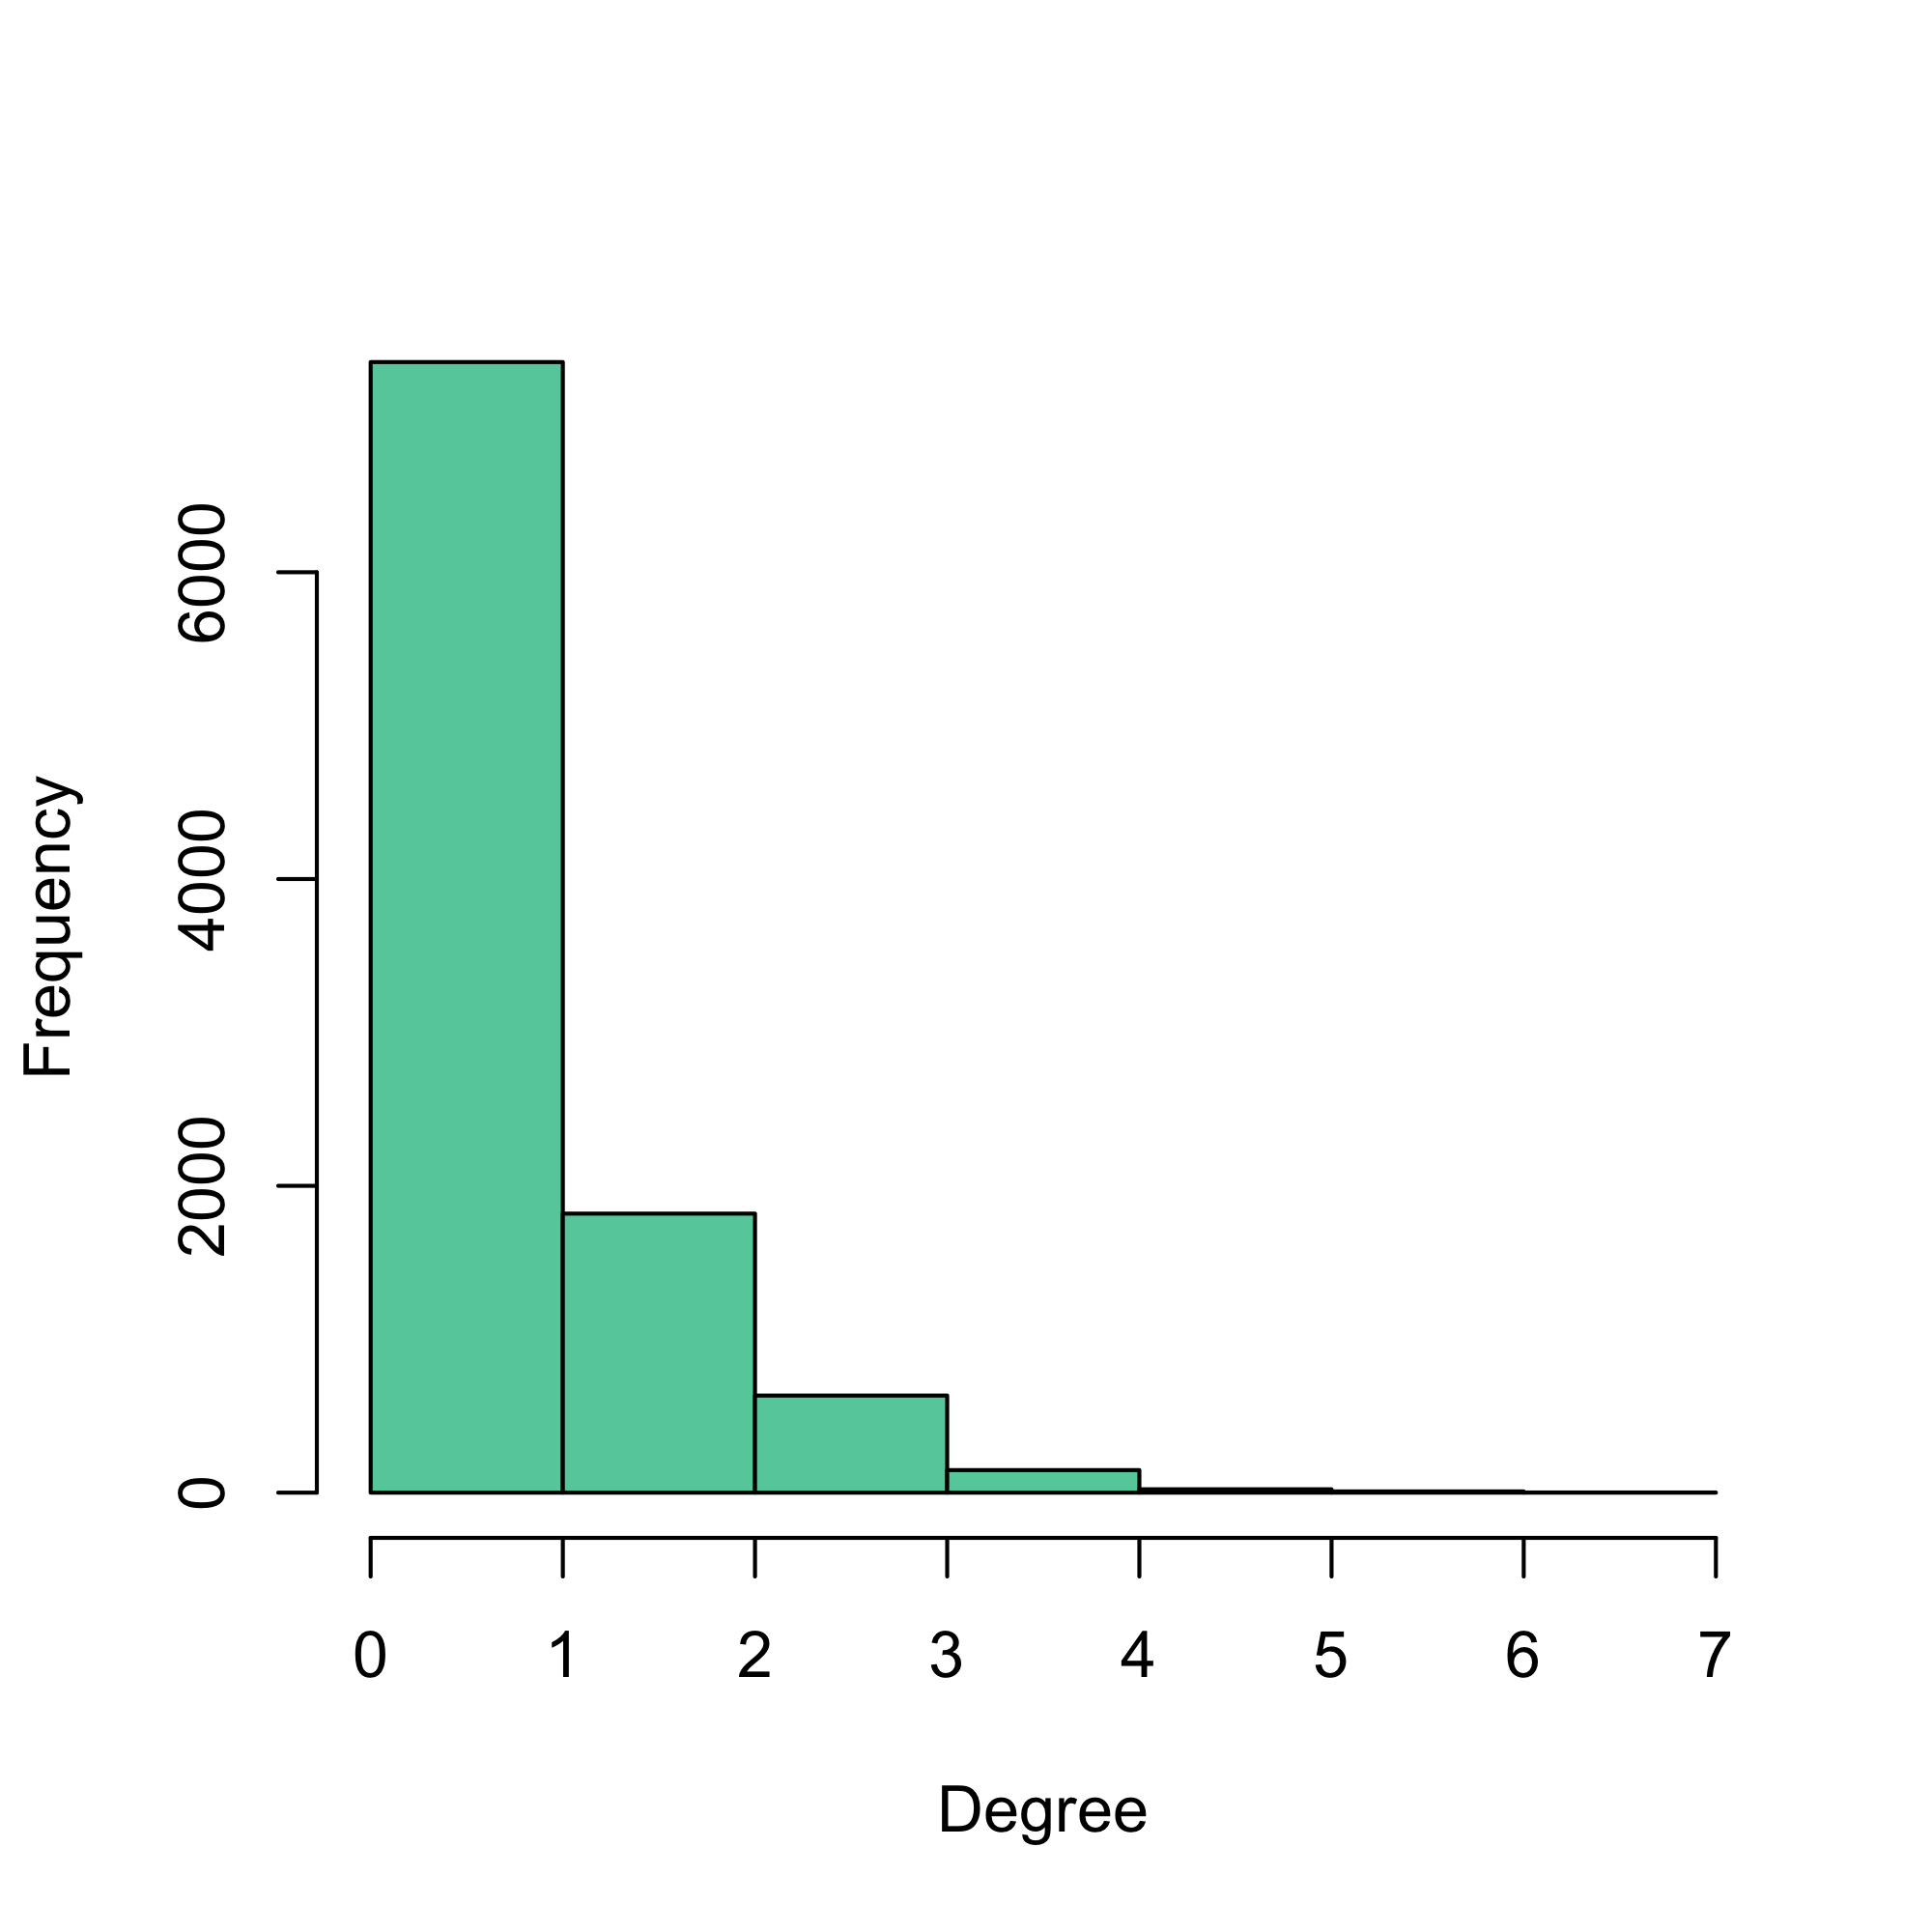
\includegraphics[width=\linewidth]{gnp_degree_histogram.png}
		\caption{Histogram of degrees in $G(10 000, \frac{1}{10 000})$ network.}
		\label{fig:gnp_degree_histogram}
	\end{subfigure}
	\hfill
	\begin{subfigure}[b]{0.45\linewidth}
		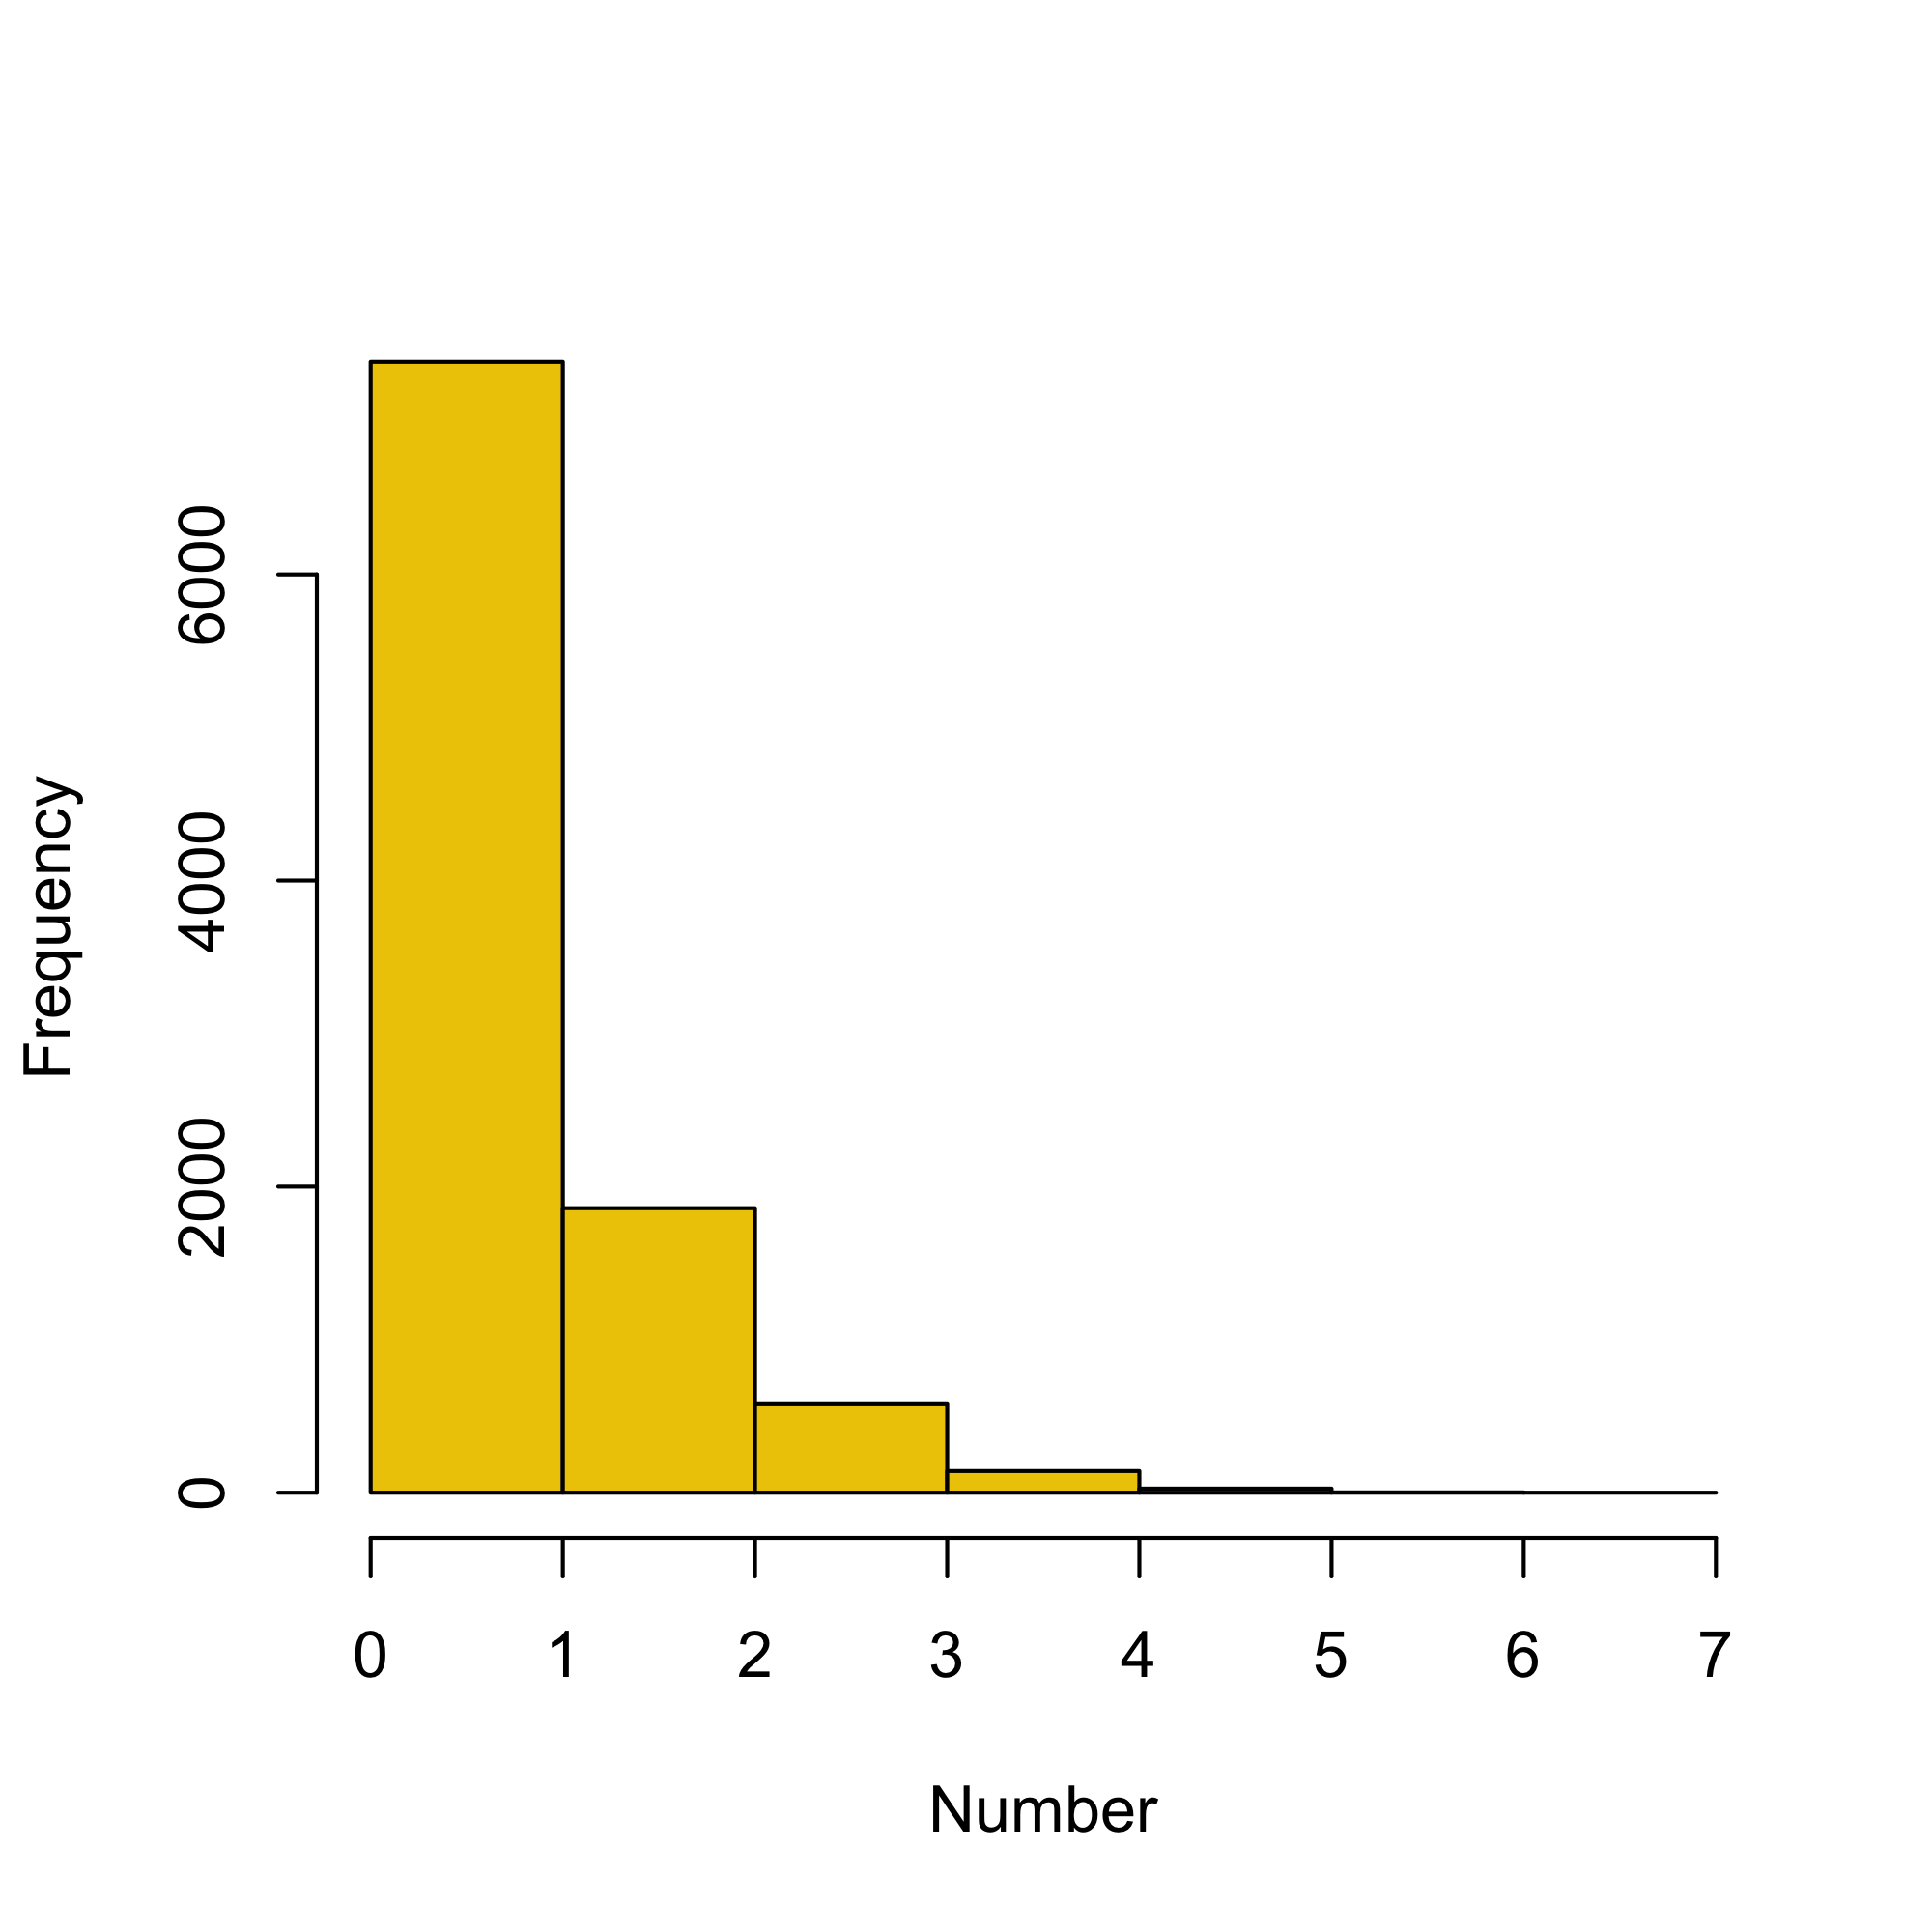
\includegraphics[width=\linewidth]{poiss_aprox_binomial.png}
		\caption{Histogram of 10 000 numbers generated by R with $\mathrm{Pois}(1)$ distribution.}
		\label{fig:poiss_aprox_binomial}
	\end{subfigure}
	\begin{subfigure}[b]{0.45\linewidth}
		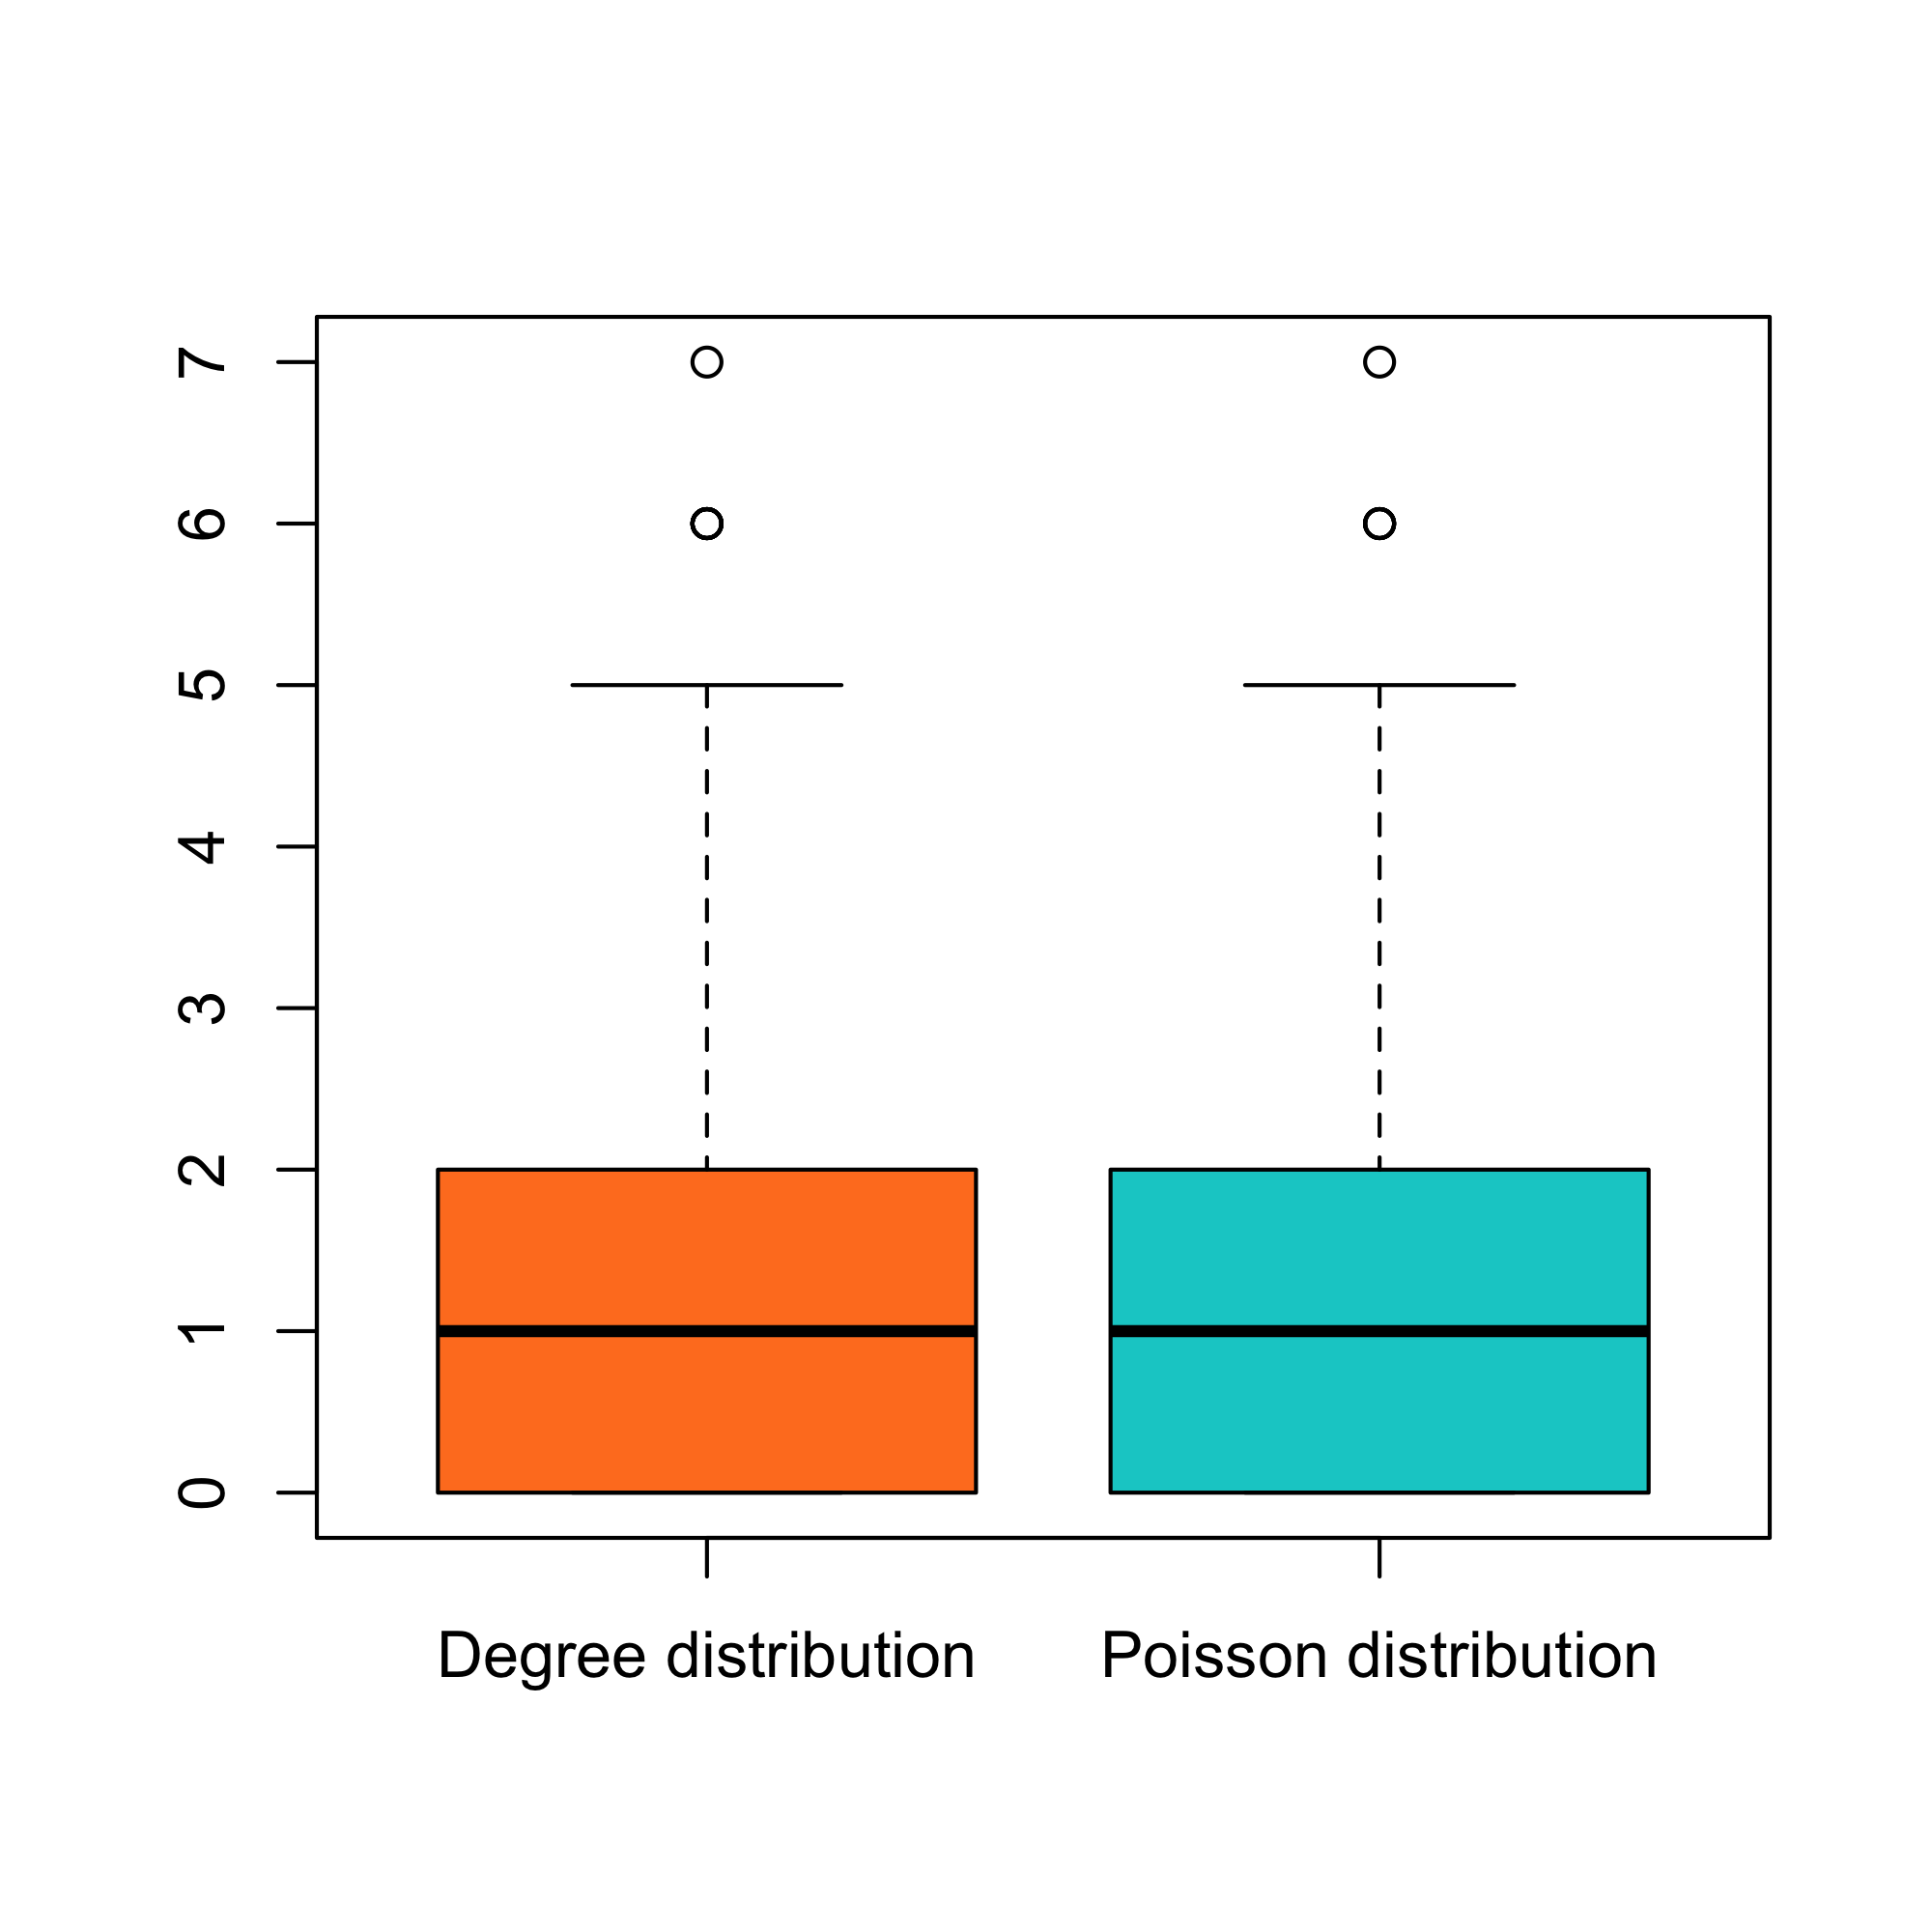
\includegraphics[width=\linewidth]{gnp_vs_poiss_boxplot.png}
		\caption{Boxplot comparing the data of Figures \ref{fig:gnp_degree_histogram} and \ref{fig:poiss_aprox_binomial}.}
		\label{fig:gnp_vs_poiss_boxplot}
	\end{subfigure}
	\caption{Degree distribution of random network and Poisson-distributed numbers.} 
	\label{fig:binom_poiss}
\end{figure}

\section{Conclusion}
This work showed how some distributions (uniform, exponential, binomial) relate to the Poisson distribution. Further work may include the relation between normal and Poisson distributions. Additionally, it may be of interest to study how to use uniform values to generate pseudo-random numbers following distributions other than Poisson.

\section{Acknowledgments}
We thank Professor Elisa Schaeffer for providing an R code with Algorithms \ref{algo:ExpAlgo} and \ref{algo:knuth}.
%%%%%%%%%%%%%%%%%%%%%%%%%%%%

\bibliographystyle{siam}
\bibliography{refr}


%%%%%%%%%%%%%%%%%%%%%%%%%%%%
\end{document}
